\documentclass[a4paper,twoside, openright,12pt]{report}
\usepackage{psfrag,amsbsy,graphics,float}
\usepackage[dvips]{graphicx, color}
\usepackage[latin1]{inputenc}
\usepackage{verbatim} 
\usepackage{appendix}

% MY CHANGE
%\usepackage[bookmarksnumbered=true]{hyperref} 

\usepackage[bookmarks=true,colorlinks=true,       % false: boxed links; true: colored links
    linkcolor=black,          % color of internal links
    citecolor=black,        % color of links to bibliography
    filecolor=black,      % color of file links
    urlcolor=black           % color of external links
]{hyperref}
 

%%% Stand 14.09.2007
%%% erstellt von Marion Sobotka
%%% marion.sobotka@tum.de
%%% last changes: 14.01.09


%_______Kopf- und Fu�zeile_______________________________________________________
\usepackage{fancyhdr}
\pagestyle{fancy}
%um Kopf- und Fu�zeile bei chapter-Seiten zu reaktivieren
\newcommand{\helv}{%
   \fontfamily{phv}\fontseries{a}\fontsize{9}{11}\selectfont}
\fancypagestyle{plain}{	
	\fancyfoot{}% keine Fu�zeile
	\fancyhead[RE]{\helv\leftmark}% Rechts auf geraden Seiten=innen; in \leftmark stehen \chapters
	\fancyhead[LO]{\helv\rightmark}% Links auf ungeraden Seiten=au�en;in \rightmark stehen \sections
	\fancyhead[RO,LE]{\thepage}}%Rechts auf ungeraden und links auf geraden Seiten
%Kopf- und Fu�zeile f�r alle anderen Seiten
\fancyfoot{}
\fancyhead[RE]{\helv\leftmark}
\fancyhead[LO]{\helv\rightmark}%alt:\fancyhead[LO]{\itshape\rightmark}
\fancyhead[RO,LE]{\thepage}
%________________________________________________________________________________


%_Definieren der R�nder und L�ngen__________
\setlength{\textwidth}{15cm}
\setlength{\textheight}{22cm}
\setlength{\evensidemargin}{-2mm}
\setlength{\oddsidemargin}{11mm}
\setlength{\headwidth}{15cm}
\setlength{\topmargin}{10mm}
\setlength{\parindent}{0pt} % Kein Einr�cken beim Absatz!!
%___________________________________________


%_______Titelseite__________________________________________
\begin{document}
\pagestyle{empty}
\enlargethispage{4.5cm} %Damit das Titelbild weit genug unten ist!
\begin{center}
\phantom{u}
\vspace{0.5cm}
\Huge{\sc Numerical Test Rig for Large-Scale and Interconnected Dynamical
Systems}\\
\vspace{1.5cm}
                                 \large{submitted\\
				  Project Laboratory\\
				  Networked and Cooperative Control\\
			  %DIPLOMARBEIT\\%/STUDIENARBEIT/MASTERRBEIT/BACHELORARBEIT\\ 
                               %            von\\
                              %  \large{Zwischenbericht zur\\
			%DIPLOMARBEIT/STUDIENARBEIT/MASTERARBEIT/
					   % BACHELORARBEIT\\ 
					   by         

						
					\begin{tabular}{c c}
					    \vspace{0.4cm} & \vspace{0.4cm} \\
					 cand. ing. Francisco Llobet& cand. ing. Jose Rivera  \\
						\vspace{0.5cm} & \vspace{0.5cm}\\
					born on July 9, 1985 & born on December 18, 1986\\
					resident: & resident:\\
					Briennerstr. 39& Amalienstr. 87\\
					80333 M\"{u}nchen & 80799 M\"{u}nchen  
					\end{tabular}

					                           
					%Tel.: +49\,176\,233\,14721\\
					\vspace{1.5cm}
					Institute of\\
					Automatic Control Engineering\\
					Technische Universit\"{a}t M\"{u}nchen\\
					\vspace{0.3cm}
					Univ.-Prof. Dr.-Ing./Univ. Tokio Martin Buss\\
                                        Univ.-Prof. Dr.-Ing. Sandra Hirche}
\end{center}
\vspace{2.5cm}
\begin{tabular}{ll}
Supervisor: & F. Deroo, S. Erhart, A. Gusrialdi, H. Mangesius  \\
Beginn: & 09.05.2011  \\
Submitted &  04.07.2011 \\
\end{tabular}
%____________________________________________________________

\newpage

%_______Abstract_____________________________________________
\topmargin5mm
\textheight220mm
\pagenumbering{arabic}
\phantom{u}
\begin{abstract}
The goal of this project was to develop a test rig for large-scale and interconnected dynamical systems. The result is
MTIDS or Matlab Toolbox for Interconnected Dynamical Systems, which is a mash-up that wraps different toolboxes used for graph analysis and 
dynamic systems simulation together. MTIDS allows the definition and analysis of graphs, where each node has a specific dynamic assign to it. 
The template based design of nodes' dynamics allows great flexibility for the creation of complex interconnected dynamical systems with the 
possibility of implementing clusters/layers. MTIDS is an open-source project under the GNU GPL v2 license. This document presents a general description 
of MTIDS and instructions for its use.    
%\vspace{2cm}
% \begin{center}
% \normalsize \textbf{Zusammenfassung}\\
% \end{center}
% Dieser Hauptseminar besch\"{a}ftigt sich mit der Methode der getriggerten Optimierung. Dabei wird besonderen Focus auf die m\"{o}glichen Anwendungen f\"{u}r Energiesystemen gesetzt.
% Als erstes wird eine Analyse der Methode in ihre genaralisierte Form f\"{u}r das NUM (Netzwerk Nutzen Maximirung) Problem durchgef\"{u}hrt. Als zweites wird ihre Anwendung an das OPF (Optimale Leistungsfluss) in Energienetzen evaluiert. Als letztes werden
% verbesserungs Vorschl\"{a}gen und weitere Anweundungen in Energiesystemen diskutiert.  
\end{abstract}
%____________________________________________________________

\newpage

%_______Widmung_______________________________________________
\phantom{u}
\phantom{1}\vspace{6cm}
\begin{center}
%Hier die Widmung oder leer lassen
\end{center}
%_____________________________________________________________



\pagestyle{fancy}

%_________Inhaltsverzeichnis__________________________
\tableofcontents 
%_____________________________________________________




%_________Einleitung__________________________________
\chapter{Introduction} \label{chapter1}

In this first Chapter the motivation behind the MTIDS project is explained and the project's goal and framework is presented.

\section{Motivation}
Large-scale interconnected dynamical system are everywhere: biological systems, power and water systems, the brain neurons, 
social interaction networks, economic markets, etc. In a canonical form all of this systems can be thought as a bunch of nodes with local dynamics 
that interact with each other, e.g. a graph. Different topologies of the graph, may lead to different behavior. An example of various 
large scale interconnected systems can be seen in Figure \ref{largePic}. 


\begin{figure}[htb]
\centering
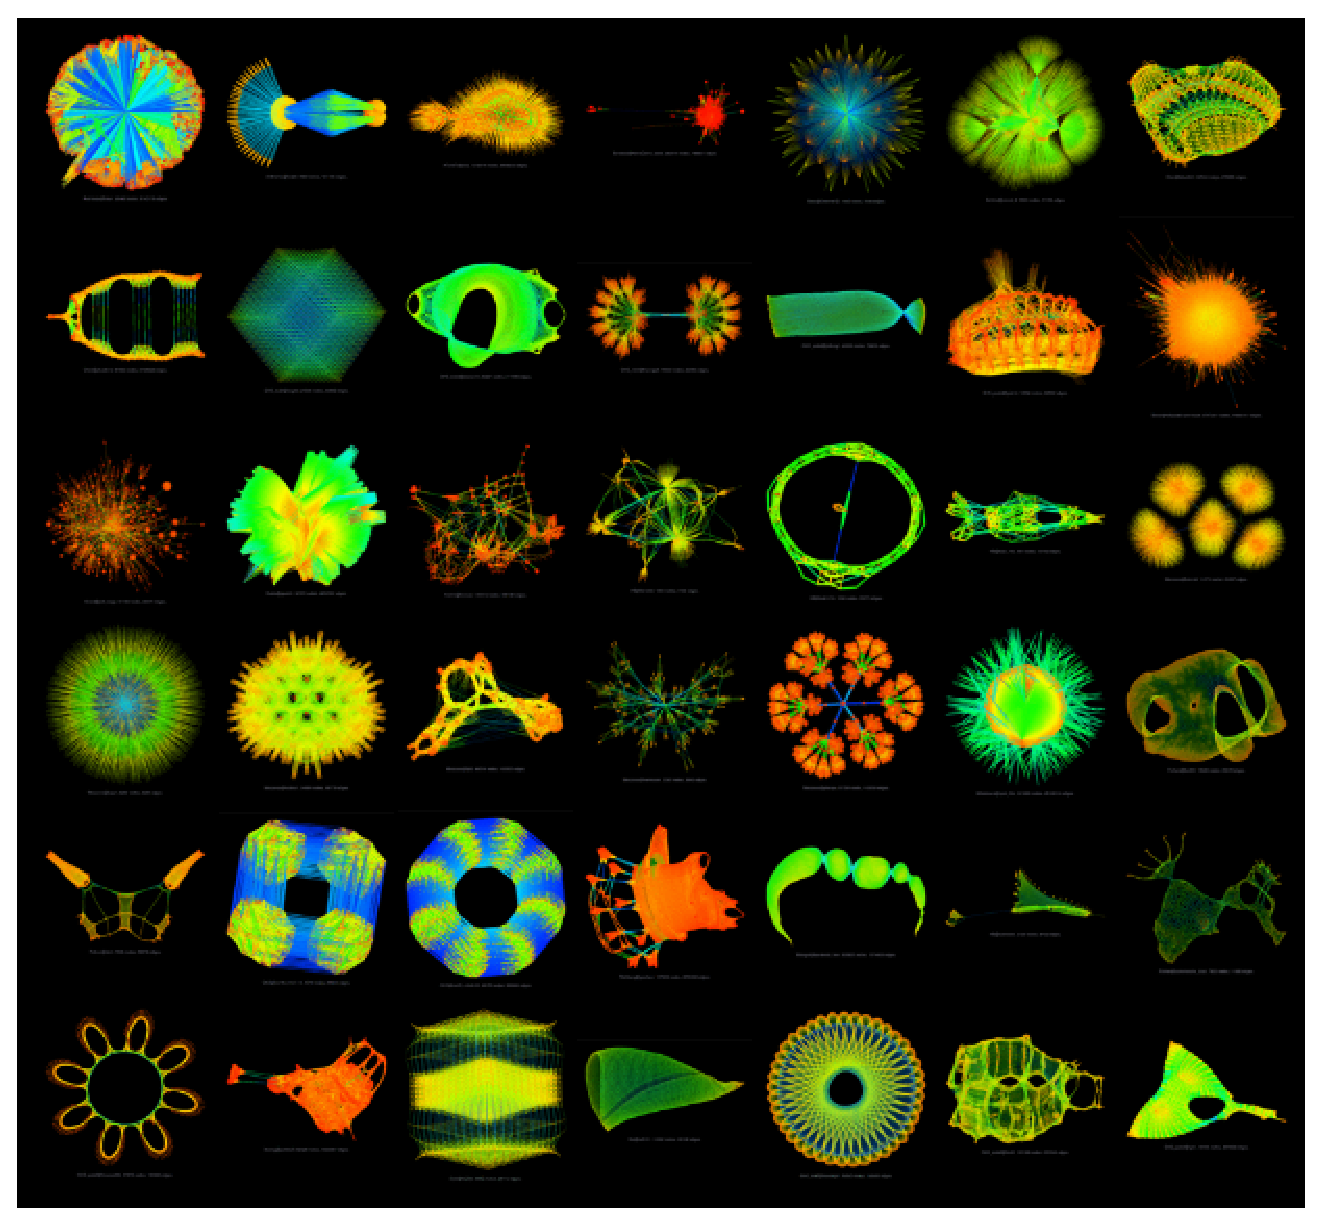
\includegraphics[width=0.5\textwidth]{pics/complex.eps}
\caption[Example of large-scale systems]{Visualization of various large scale systems using the sfdp algorithm $\copyright$ Dr. Yifan Hu of AT\&T Labs}
\label{largePic}
\end{figure}

There are many tools available for the analysis of interconnected dynamical systems, for example in power systems you have PSSE and Power Factory. However,
this simulation programs are normally very system specific and in most cases it takes a long time to learn how to use them correctly. 
The difficulties are specially noticed while
testing control concepts, where small changes on the topology of the grid or control concept could lead to a painful redesign of your simulation set up. 
You may actually end up spending the most of your time in the implementation of a simulation. A more general and 
easy to use solution for the simulation of interconnected dynamical systems is needed.




\section{Idea and Goal}

\textbf{MTIDS} (Matlab Toolbox for Interconnected Dynamical Systems) is a project that aims to design an easy 
to use and flexible toolbox to make the simulation of large scale dynamical systems easier for students and researchers. 
The \textbf{goal} is to produce a mash-up that wraps different toolboxes used for graph analysis and 
dynamic systems simulation together into a framework.  


\begin{figure}[htb]
\centering
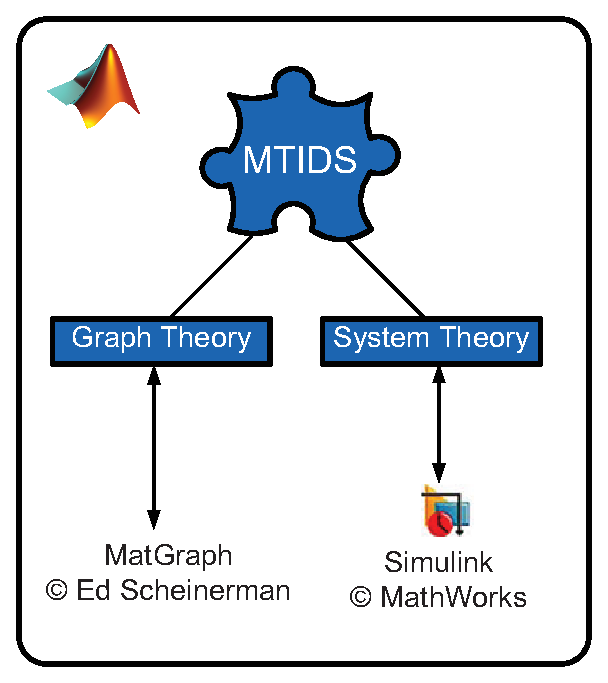
\includegraphics[width=0.5\textwidth]{pics/mtidsStructure.eps}
\caption[MTIDS idea]{MTIDS: Matlab Toolbox for Interconnected Dynamical Systems}
\label{mtidsFig}
\end{figure}

As we can see in Figure \ref{mtidsFig} MTIDS runs in the MATLAB environment and is basically a GUI that allows the interaction of tools used in graph theory 
and control theory.  For graph theory we use Matgraph a toolbox design by Prof. Scheinerman of the John Hopkins University and for dynamical simulations
we use Simulink. 

\section{Framework}

The current framework of MTID is made out of three basic components. A GUI (\textbf{mtids.m}) an export to simulink function (\textbf{exportSimulink.m}) and
an import from Simulink function (\textbf{importSimulink.m}).\\

 

\begin{figure}[htb]
\centering
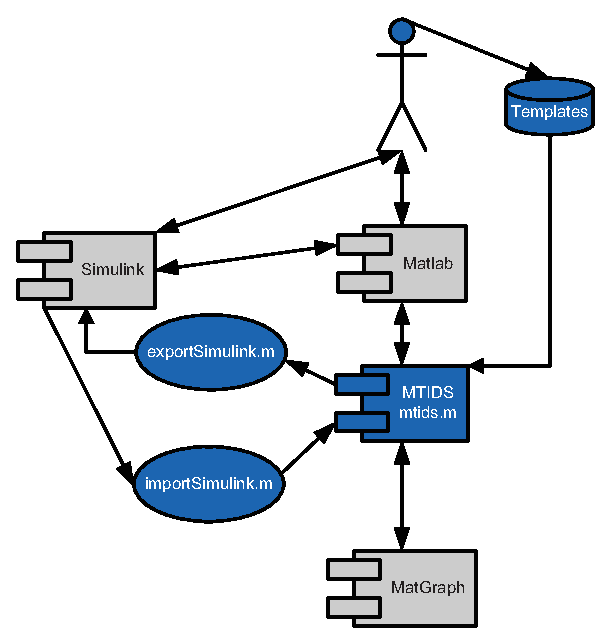
\includegraphics[width=0.5\textwidth]{pics/uml.eps}
\caption[MTIDS components]{MTIDS: Components diagram}
\label{componentsFig}
\end{figure}

In Figure \ref{componentsFig} we can see that the most important component is the user, specially its head. The better you are at producing templates
and interacting with matlab and simulation the more functional MTIDS is going to be for you.
In a nutshell MTIDS works as follows:
\begin{itemize}
\item GUI (mtids.m) runs inside Matlab
\item GUI interacts with Matgraph: create, modify and visualize graphs  
\item System Inteconnector (SI): exportSimulink.m and importSimulink.m called from GUI to interact with Simulink
\item Templates done by User in Matlab/Simulink.
\item Simulations done in Simulink
\end{itemize}
%  
% 
% The GUI (mtids.m) runs inside matlab. The UI interacts 
% with Matgraph to create, modify and visualize graphs. The ystem Inteconnector (SI) compose of the functions exportSimulink.m and importSimulink.m are
% called from GUI to interact with Simulink. The user can define the nodes dynamic by building custom templates in Matlab/Simulink. The simulations are
% ultimately done in Simulink.

%%%%%%%%%%%%%%%%%%%%%%%%%%%%%%%%%%%%%%%%%%%%%%%%%%%%%% GRAPH
\chapter{Graph Theory}\label{chapter2}



%_%%%%%%%%%%%%%%%%%%%%%%%%%%%%%%%%%%%%%%%%%%%%%%%%%%%%%%%%%%%%%%%%%%%%%%%%%%%%%%%%%%%%%%%%%% SYSTEM_____________________________________
\chapter{System Theory}\label{chapter3}

In this Chapter we explain the design and simulation capabilities that MTIDS offers for interconnected dynamical systems.

\section{MTIDS Concepts for Simulink Models} \label{subsystemConcept}
\subsection{Nodes and connections}
\subsubsection{Node:}
Each node in MTIDS is a subsystem block in Simulink. Each node must have a unique label.
Each node has an in-port for every node in the graph and an out-port. 
\subsubsection{Connections:}
Any connection made inside MTIDS is bidirectional and unweighted. As Simulink connections are directed, each MTIDS bidirectional connection
 is represented with two directed connections between nodes. To implement weighted graphs, weights 
on branches have to be realized in the node's dynamic model, e.g inside the subsystem. Another option is to define junction nodes.

\section{Export to Simulink}\label{exportToSimulink}
In order to export the model created in the MTIDS GUI to simulink: \textbf{Simulation $\rightarrow$ Export to Simulink...} (see Figure \ref{exportFig})
\\
\begin{figure}[htb]
\centering
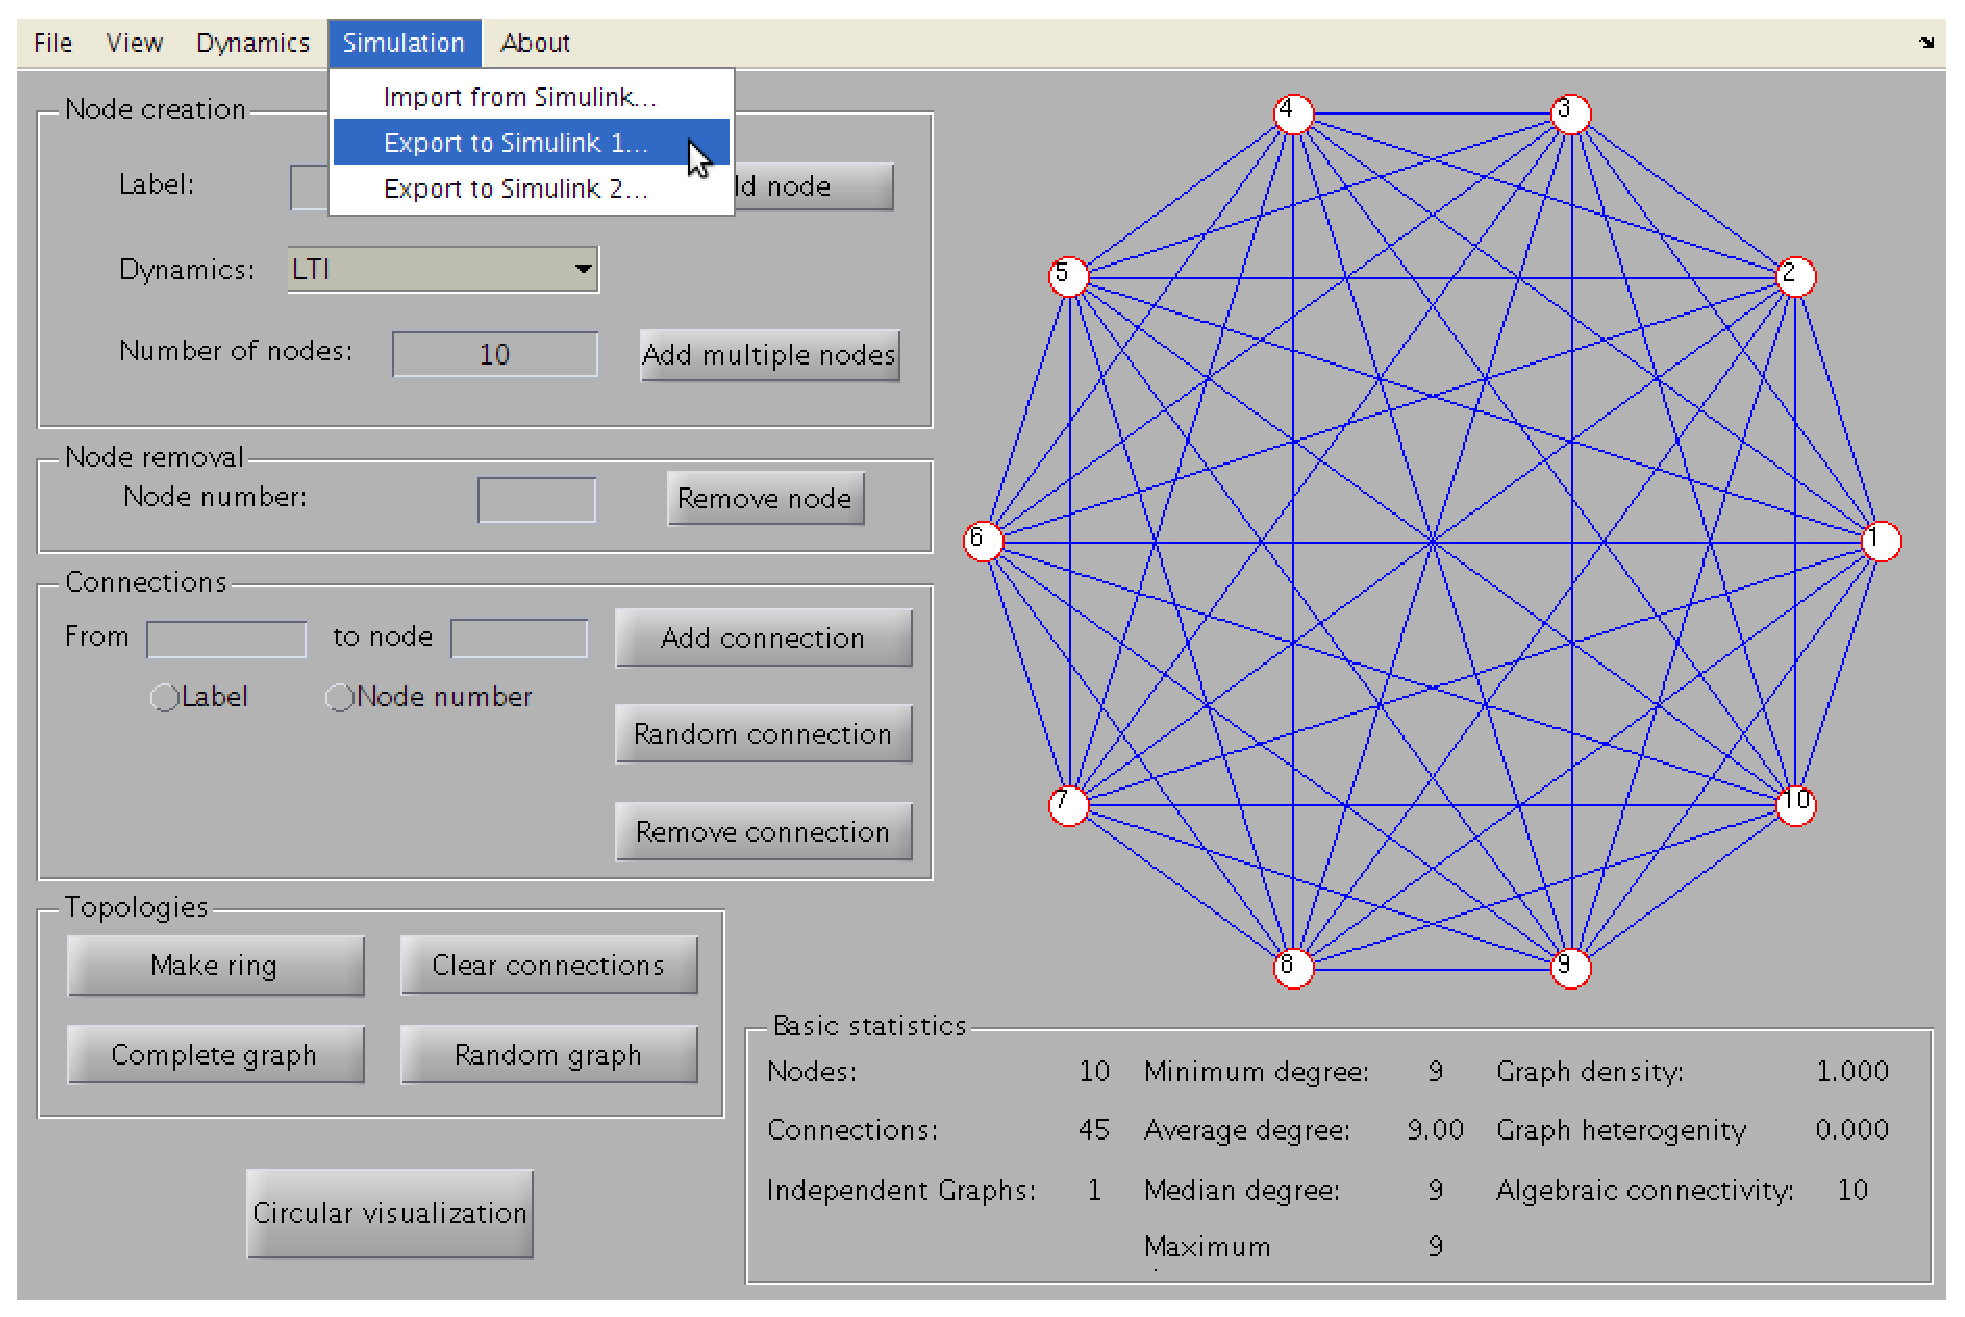
\includegraphics[width=0.7\textwidth]{pics/screenExport.eps}
\caption[MTIDS export to Simulink]{MTIDS: export model to Simulink. Example is a complete graph with 10 LTI nodes. }
\label{exportFig}
\end{figure}

The MTIDS GUI then calls the function exportability.m which builds a Simulink model with the following information:
model name, list of nodes' dynamics templates, list of templates that are available in mtids, adjacency matrix, position of the nodes and nodes' names. 
The result is a Simulink model in the MTIDS format. \\

To adjust the size of the model to the Simulink window size: \textbf{View $\rightarrow$ Fit System To View}\\
% 

\begin{figure}[htb]
\centering
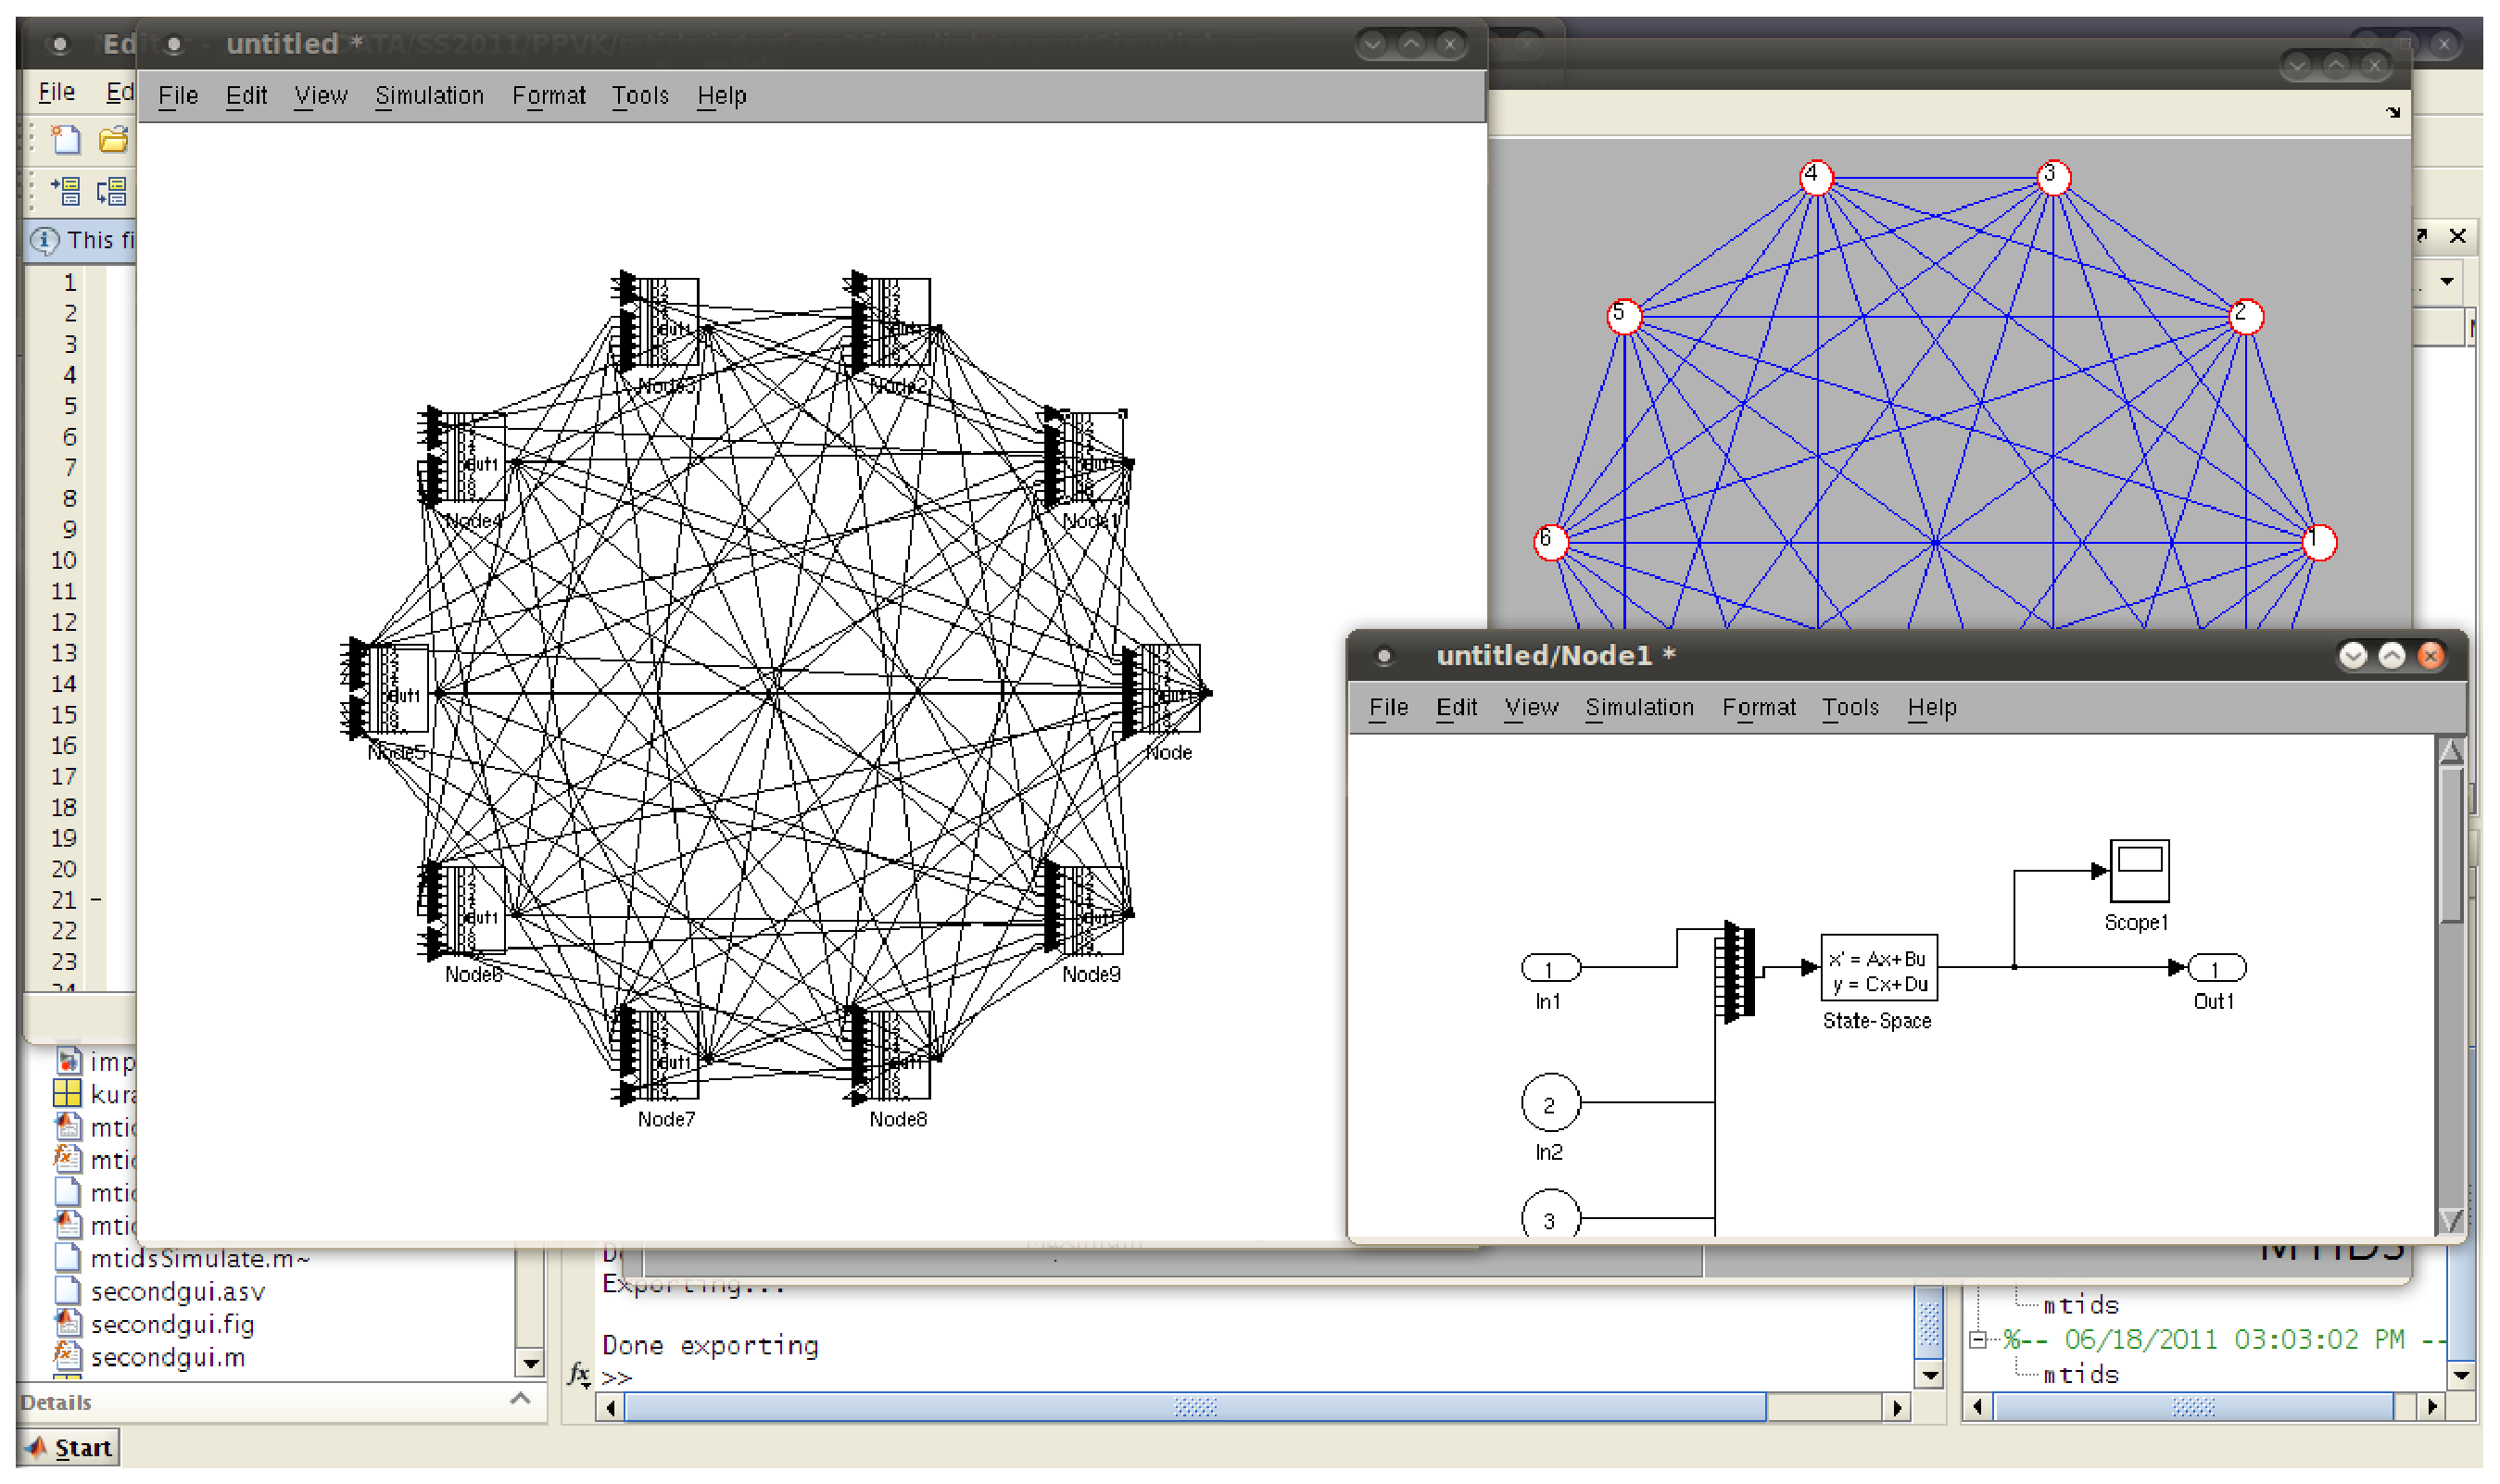
\includegraphics[width=0.7\textwidth]{pics/screenExportResult.eps}
\caption[MTIDS exported Simulink model]{Interconnected system Simulink Model. Example is a complete graph with 10 LTI nodes. }
\label{exportFig}
\end{figure}

In Figure \ref{exportFig}, the nodes are ordered in a circle, the topology of the system defined in MTIDS remains. The circle arrangement is a 
design decision, made, in order to allow a better access to the nodes. Each one of the nodes is a subsystem block. The dynamic of the nodes is defined inside
the subsystem block. Moreover, each node has a single out-port and N in-ports, where N is the number of nodes the whole system has. Each node on the 
system has its own in-port on each node, compare with a zoom on the first node of our example in Figure \ref{nodeFig}. \\
 
\begin{figure}[htb]
\centering
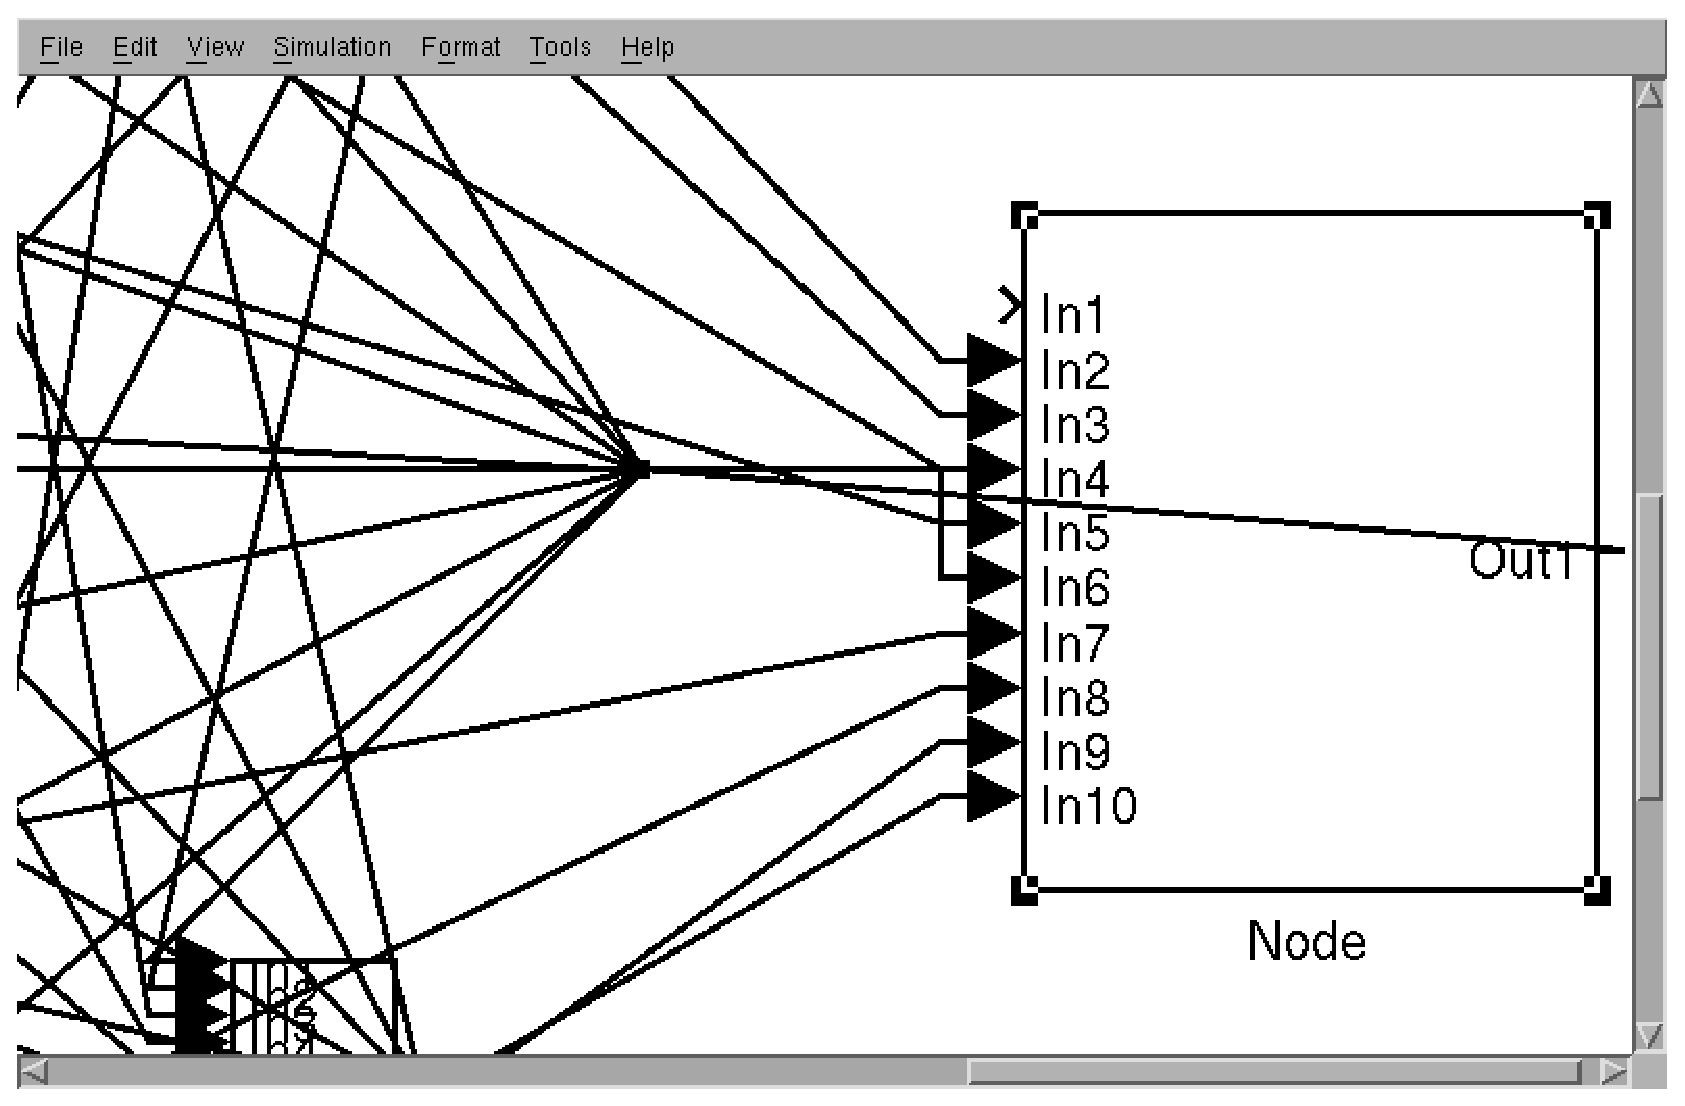
\includegraphics[width=0.5\textwidth]{pics/screenNode.eps}
\caption[MTIDS node in Simulink]{Node inputs and output: Each node has an in-port for every node in the model and an out-port. Example is the first node of a complete graph with 10 LTI nodes. }
\label{nodeFig}
\end{figure}
Notice that the port corresponding to the nodes number
should always be free, e.g. the first node has an unconnected in-port 1, the second node an unconnected in-port 2, etc. 
In case that a loop of a node with itself is required we recommend doing this inside the subsystem/node. 
Another important aspect to point out is that when simulating the system, Simulink will issue a warning for unconnected in-ports and set their input to the subsystem to 0, this means 
that an \textbf{unconnected port enters the subsystem (local dynamics of the node) with a value of zero} during simulations. This can be exploited to 
make the parametrization of the nodes' dynamics easier. 

\section{Nodes' Dynamics}

As mentioned in the past section \ref{exportToSimulink} each node defined in MTIDS is exported to Simulink as a subsystem. The exportSimulink.m function 
uses predefined dynamic templates, which are modified according to the, in MTIDS, defined topology. Next, we explain how to define your own templates and
show how to use 2 preloaded templates: the LTI template and the kuramoto template. 


\subsection{Build your own Template} \label{nodeTemplate}
The real power of MTIDS depends on your ability to build templates. 
\\
\begin{figure}[htb]
\centering
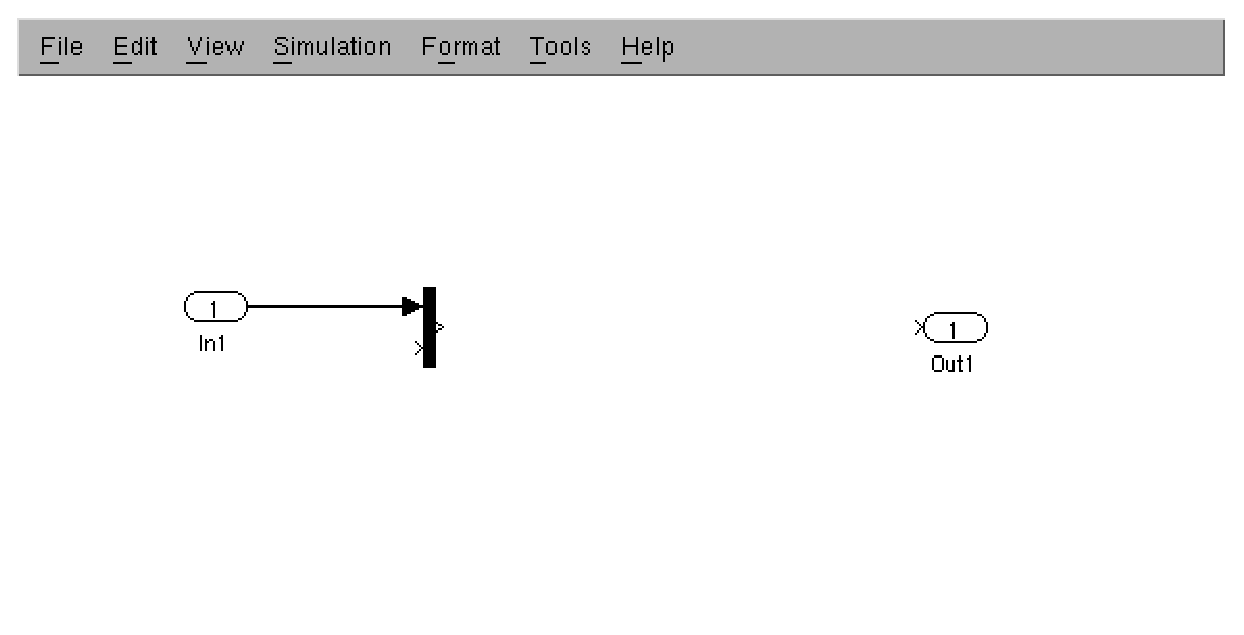
\includegraphics[width=0.6\textwidth]{pics/screenBuildTemplate.eps}
\caption[MTIDS Dynamics Template]{Scratch template for node's dynamics.}
\label{templateFig}
\end{figure}

In Figure \ref{templateFig} we can see the components that each template should have: an in-port connected to a mux and an out-port.
Between the mux and the out-port you can design your own custom dynamics. The input to the system comes from mux as vector, which is composed by the values
entering the node/subsystem. The output of your system should also be aggregated to a vector and routed to the out-port. The separation of the different inputs and outputs 
is left to the system designer. With a well thought architecture complex systems are very easy to achieve, please refer to the LTI and kuramoto template examples.  
\\

The dynamic of a node can be as simple as a junction that only reroutes the incoming signals or more complicated to include controllers and systems inside of it. It is this feature that allows
the implementation of clusters or layered systems, see subsection \ref{layering}. 


\subsection{The LTI template}

The LTI template is an example that defines a linear time invariant dynamic for nodes. The mathematical model 
of a simple interconnected LTI system is written as:
\begin{eqnarray}
\left( \begin{array}{c}
\dot{x_1} \\  
\vdots \\
\dot{x_N}
\end{array} \right)=
\left( \begin{array}{ccc}
A_{11} & \cdots & A_{1N} \\  
\vdots & \ddots & \vdots\\
A_{N1} & \cdots &A_{NN}
\end{array} \right) 
\left( \begin{array}{c}
x_1 \\  
\vdots \\
x_N
\end{array} \right)+
\left( \begin{array}{c c c}
B_{1} & \cdots & B_{N}  
\end{array} \right) 
\left( \begin{array}{c}
u_1 \\  
\vdots \\
u_N
\end{array} \right)       
\end{eqnarray}
or
\begin{equation}
 \dot{x}=Ax+Bu
\end{equation}
The local view of a single subsystem/node (here for the first node) is:
\begin{eqnarray}
  \dot{x_1}= 
\left( \begin{array}{c c c c c c c}
A_{11} & A_{12} & \cdots & A_{1N} & B_{1} & \cdots & B_{N}  
\end{array} \right) 
\left( \begin{array}{c}
x_1 \\ 
x_2 \\ 
\vdots \\
x_N\\
u_1 \\  
\vdots \\
u_N
\end{array} \right)    
\end{eqnarray}
this can be reformulated as
\begin{eqnarray} \label{LTIFor}
 \dot{x_1}= A_{11}x_1 +  
\left( \begin{array}{c c c c c c c}
A_{11} & A_{12} & \cdots & A_{1N} & B_{1} & \cdots & B_{N}  
\end{array} \right) 
\left( \begin{array}{c}
0 \\ 
x_2 \\ 
\vdots \\
x_N\\
u_1 \\  
\vdots \\
u_N
\end{array} \right) 
\end{eqnarray}





In order to keep things simple, we define the local output of each node:
\begin{eqnarray}
 y_i=  x_i,\ i=1,\ldots,N. 
\end{eqnarray}

To implement this dynamic as a template we make use of the State-Space block.

\begin{figure}[htb]
\centering
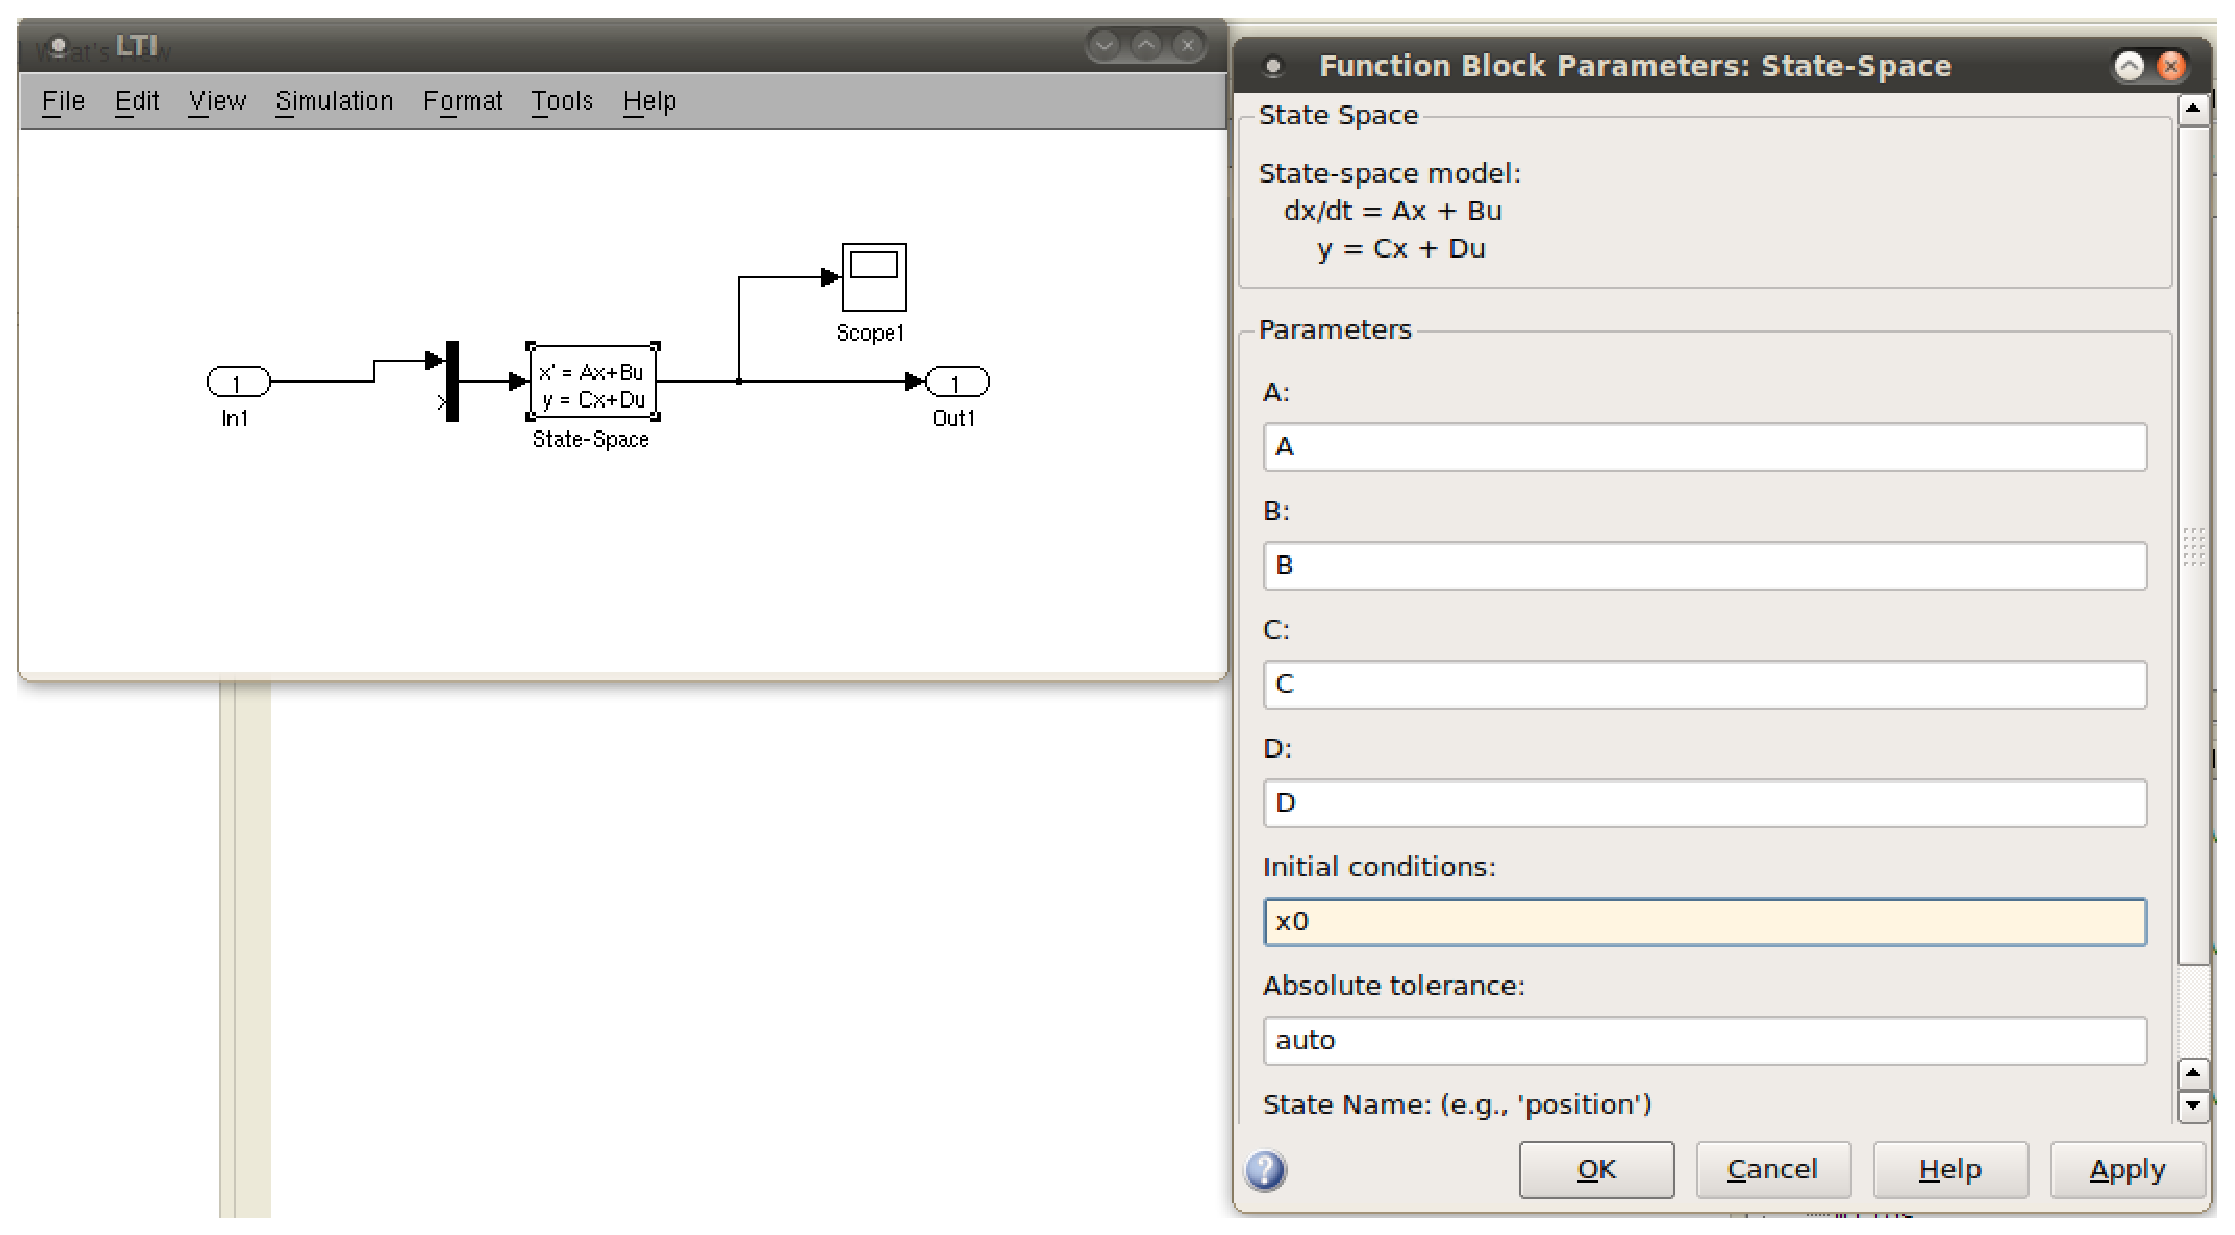
\includegraphics[width=0.8\textwidth]{pics/screenLTI.eps}
\caption[MTIDS LTI Template]{LTI template}
\label{templateLTIFig}
\end{figure}
 
This template shown in \ref{templateLTIFig} can be used in MTIDS to create interconnected LTI systems with different topologies. One way to avoid 
the work of parameterizing the A,B,C and D matrix of every node separately is to define the same matrix for all subsystems. One can use the formula 
\ref{LTIFor} and define the same A, B, C, and D matrix for every node. An example of this is
\begin{eqnarray}
 A&=& 1\nonumber\\
B&=&[-1 \cdots -1]^{1\times N}\nonumber\\
C&=& 1\nonumber\\
D&=& [0 \cdots 0] ^{1\times N}\nonumber
\end{eqnarray}

As the in-port corresponding to the node itself is automatically set to zero by Simulink during the simulation, we can define the same matrices for all 
nodes without getting any errors.
\\

For more complicated LTI models we recomend creating many different LTI templates.

\subsection{The Kuramoto Template}
The kuramoto template is an example of a non-linear dynamic for a node. The kuramoto model is used to model the behavior of coupled oscillators. One of the interesting behaviors
that may occur in this type of systems is synchronization. The mathematical equation of $N$ coupled oscillators is written for each oscillator $i$ as
\begin{equation}\label{kuramotoFor}
 \dot{\theta_i} = \omega_i + \frac{K}{N} \sum_{j=1}^N \sin(\theta_j-\theta_i). 
\end{equation}



\begin{figure}[htb]
\centering
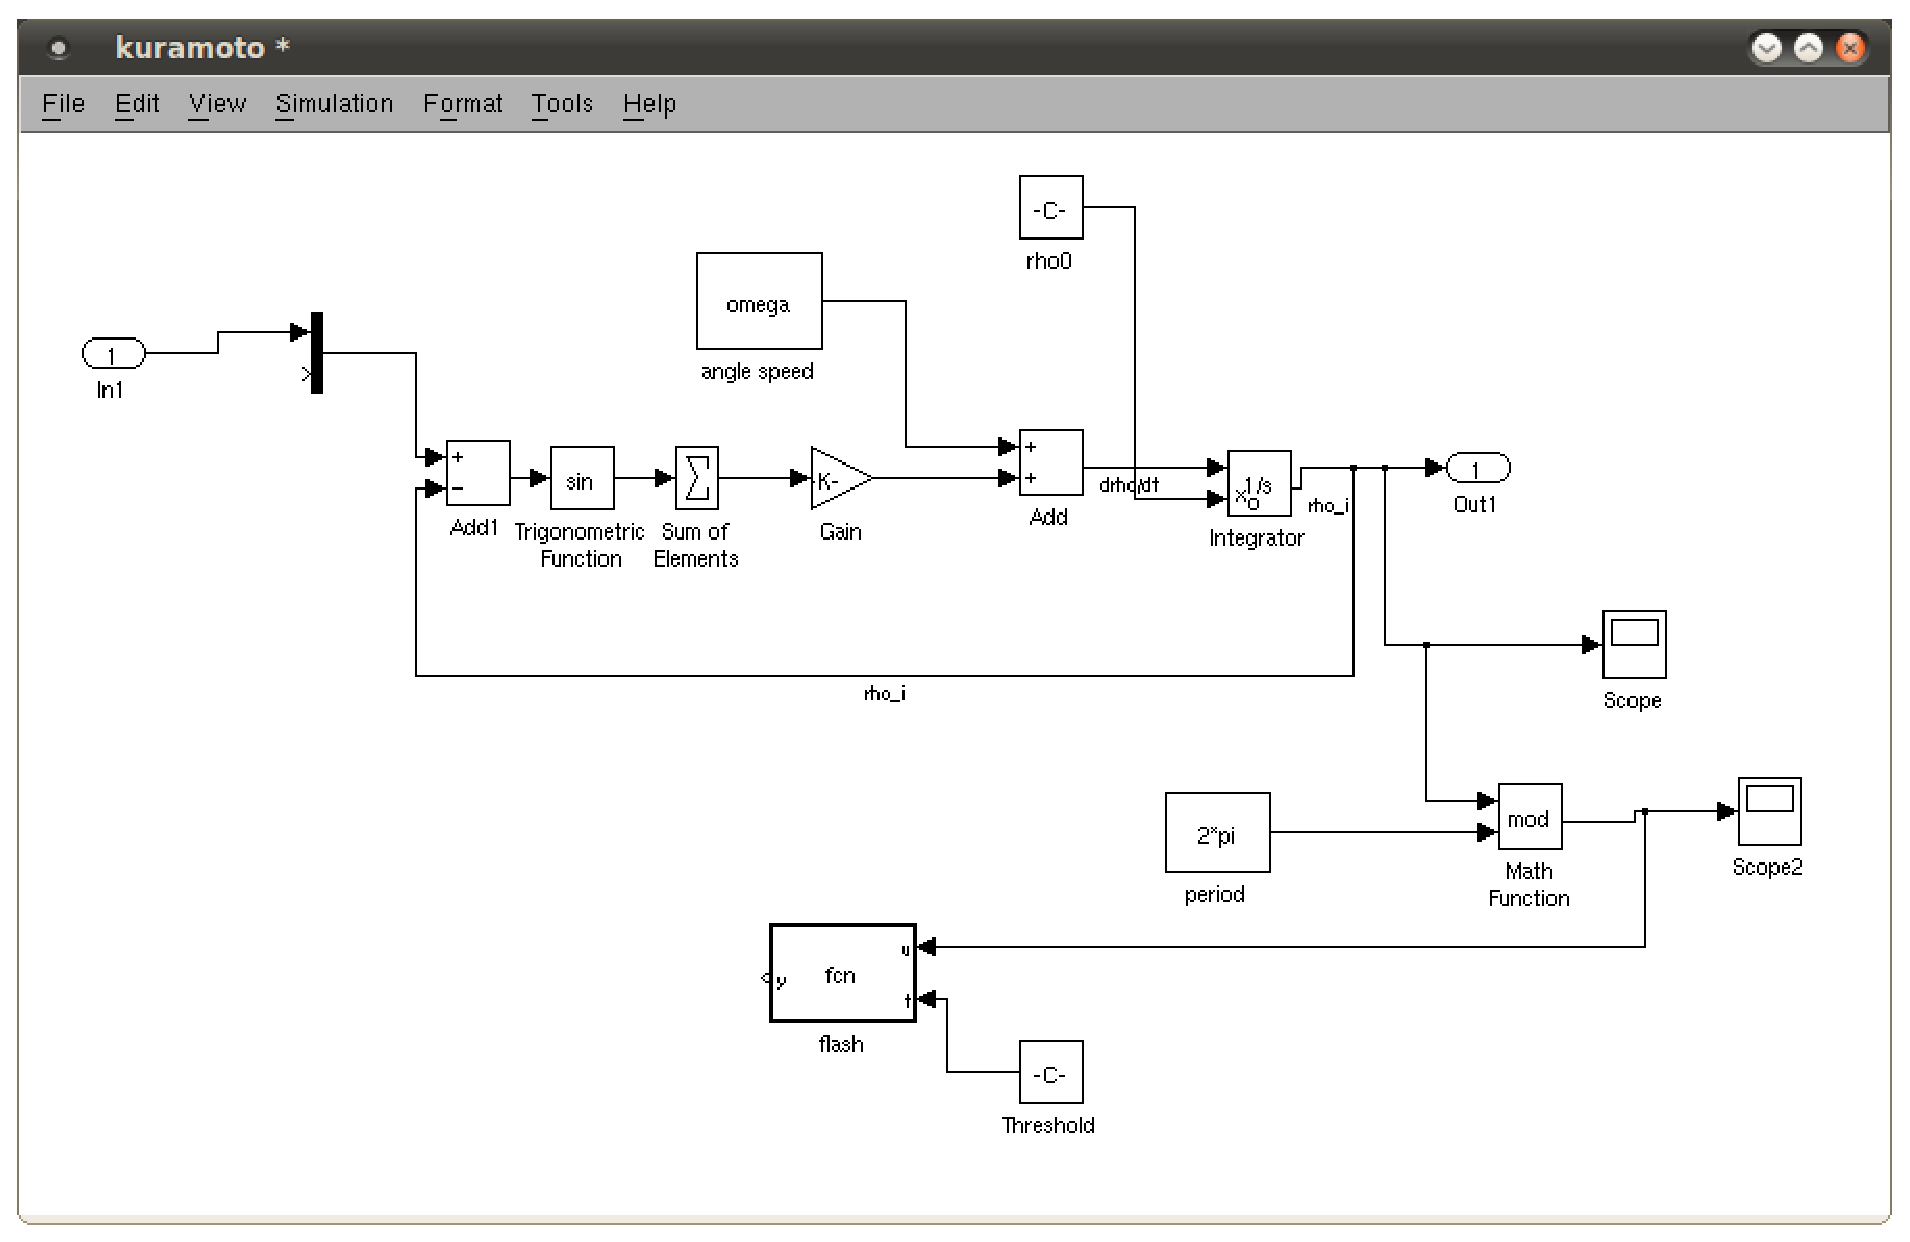
\includegraphics[width=0.7\textwidth]{pics/screenKuramoto.eps}
\caption[MTIDS Kuramoto Template]{Kuramoto template for fireflies synchronization}
\label{templateKuramotoFig}
\end{figure}
 
In Figure \ref{templateKuramotoFig} we see  the MTIDS's kuramoto template after formula \ref{kuramotoFor}. The goal was to produce fireflies synchronization, thus
the model has an embedded function that changes the color of the parent block for a defined threshold, this mimics the flashing of a firefly.
With the right parameters one can build a synchronizing firefly colony using MTIDS. Remember that the kuramoto.mdl template needs to be added in MTIDS:
Dynamics $\rightarrow$ Add mdl template. You also need to set up the right parameters for synchronization, an example can be seen in Figure \ref{syncFig}.
In order to see the blinking in the correct time scale, you need to set up the simulation with a fixed step size in Simulink, more on this in section 
\ref{workinginsimulink}.



\begin{figure}[htb]
\centering
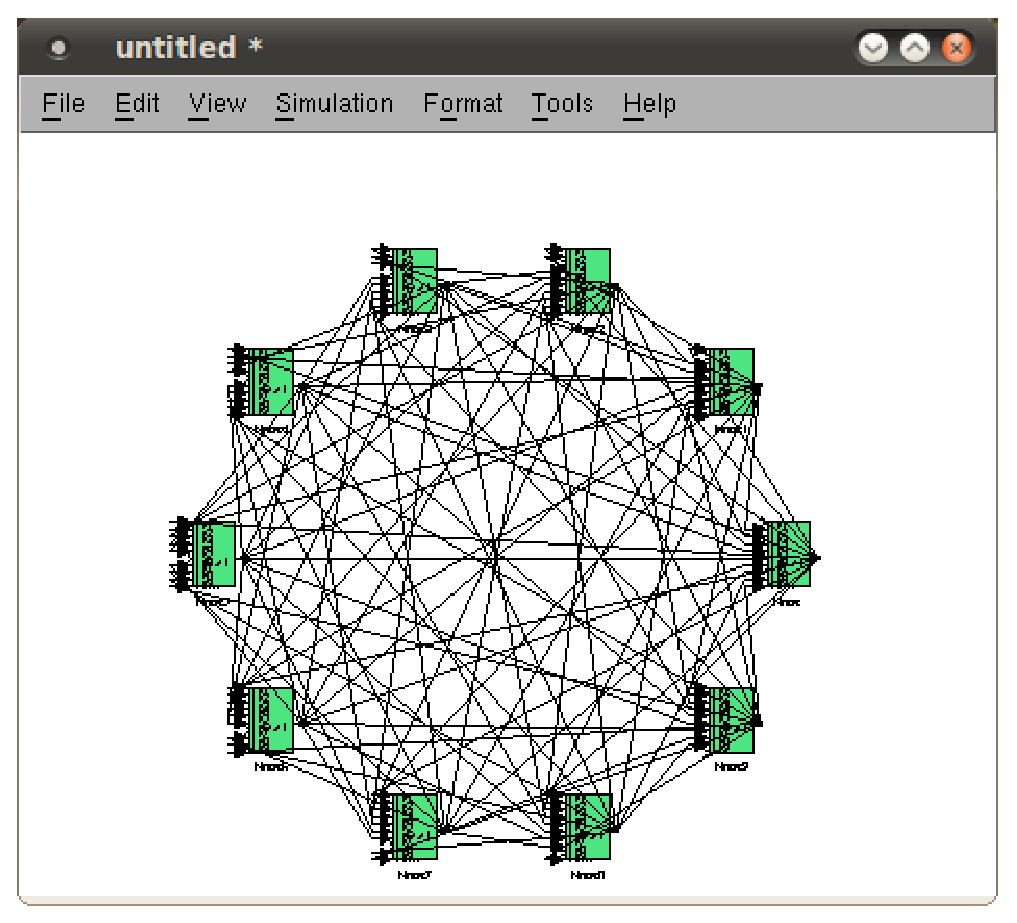
\includegraphics[width=0.5\textwidth]{pics/screenfireflies.eps}
\caption[MTIDS fireflies synchronization]{Simulation of 10 fireflies synchronizing. Parameters: K=0.1, N=10, $\omega=0.5$, $\theta_0=10$, var=5 (variation of starting point), threshold= $3/4*2\pi$}
\label{syncFig}
\end{figure}



\section{Layering/Clustering Nodes} \label{layering}


The \textbf{key} to implement layering and clustering in MTIDS is the \textbf{interface node}. On clustered/layered interconnected systems there is always an interface
that regulates the data communication of one layer/cluster to other layers/clusters. The interface has access to all nodes in the current cluster/layer and 
on most cases does some information processing (compression, principal component extraction, etc). This processed information is used to interact with 
other clusters/layers. Inside the cluster/layer the interface node acts like a normal node.
\\

\subsection{Crate a layer/cluster}

In oder to create a layer/cluster in MTIDS you need to export your system as a layer: \textbf{File $\rightarrow$ Export as a layer}.
MTIDS will ask you to select a template for the interface node. You may select a customize interface node created by you or select the MTIDS provided
interface node : \textbf{layerInterface.mdl}.\\
The result is a Simulink model that differs from the one that MTIDS normally produces, as it includes an extra node, the interface node.
If we look more closely in Figure \ref{layerFig}, we notice that this model also fulfills the requirements needed to build a standard node template, see subsection \ref{nodeTemplate}.
By saving this model and using it as a node template in MTIDS we build many of this interconnected systems which interact with each other through their 
interface nodes, see Figure \ref{layersFig}.


\begin{figure}[htb]
\centering
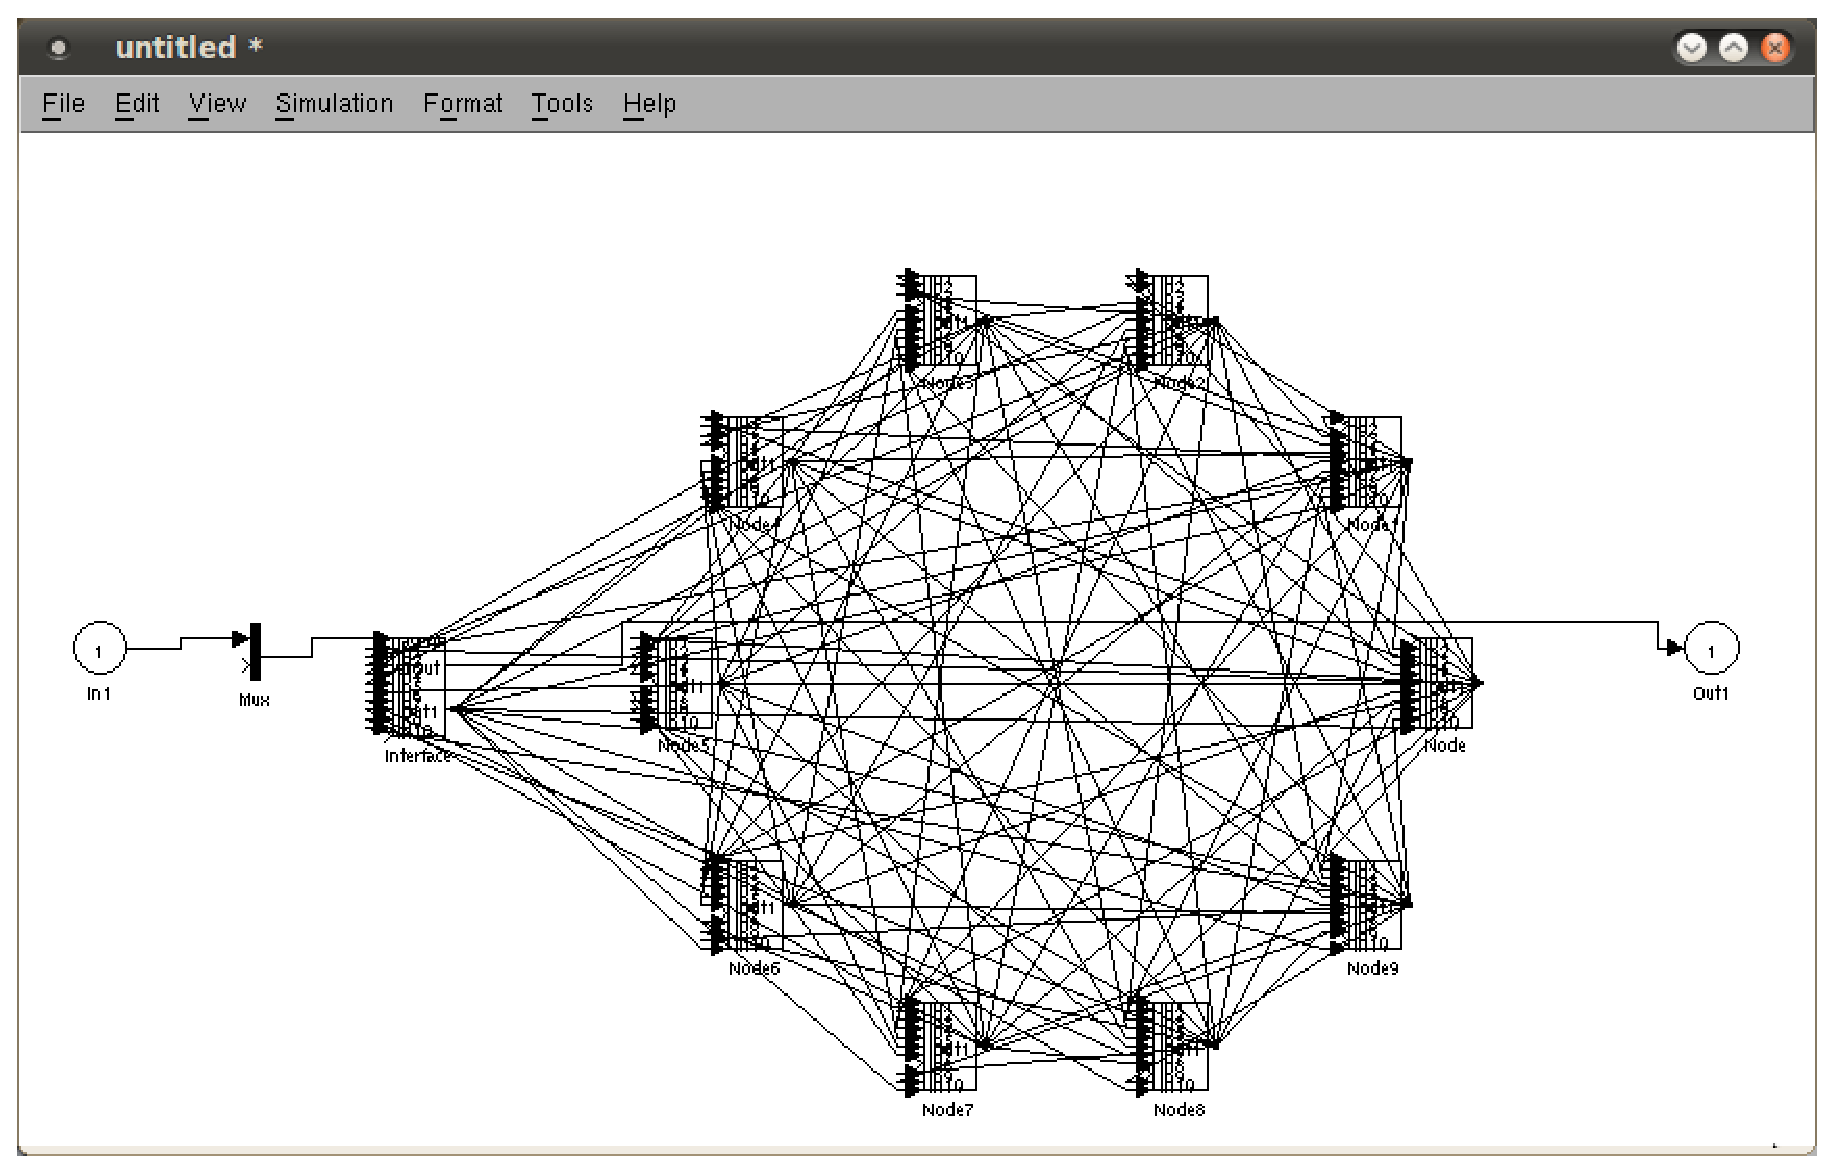
\includegraphics[width=0.5\textwidth]{pics/screenLayer.eps}
\caption[MTIDS export as layer resulting model]{Resulting layer/cluster when exporting in MTIDS as layer. Example is a complete graph with 10 LTI nodes.}
\label{layerFig}
\end{figure}



\begin{figure}[htb]
\centering
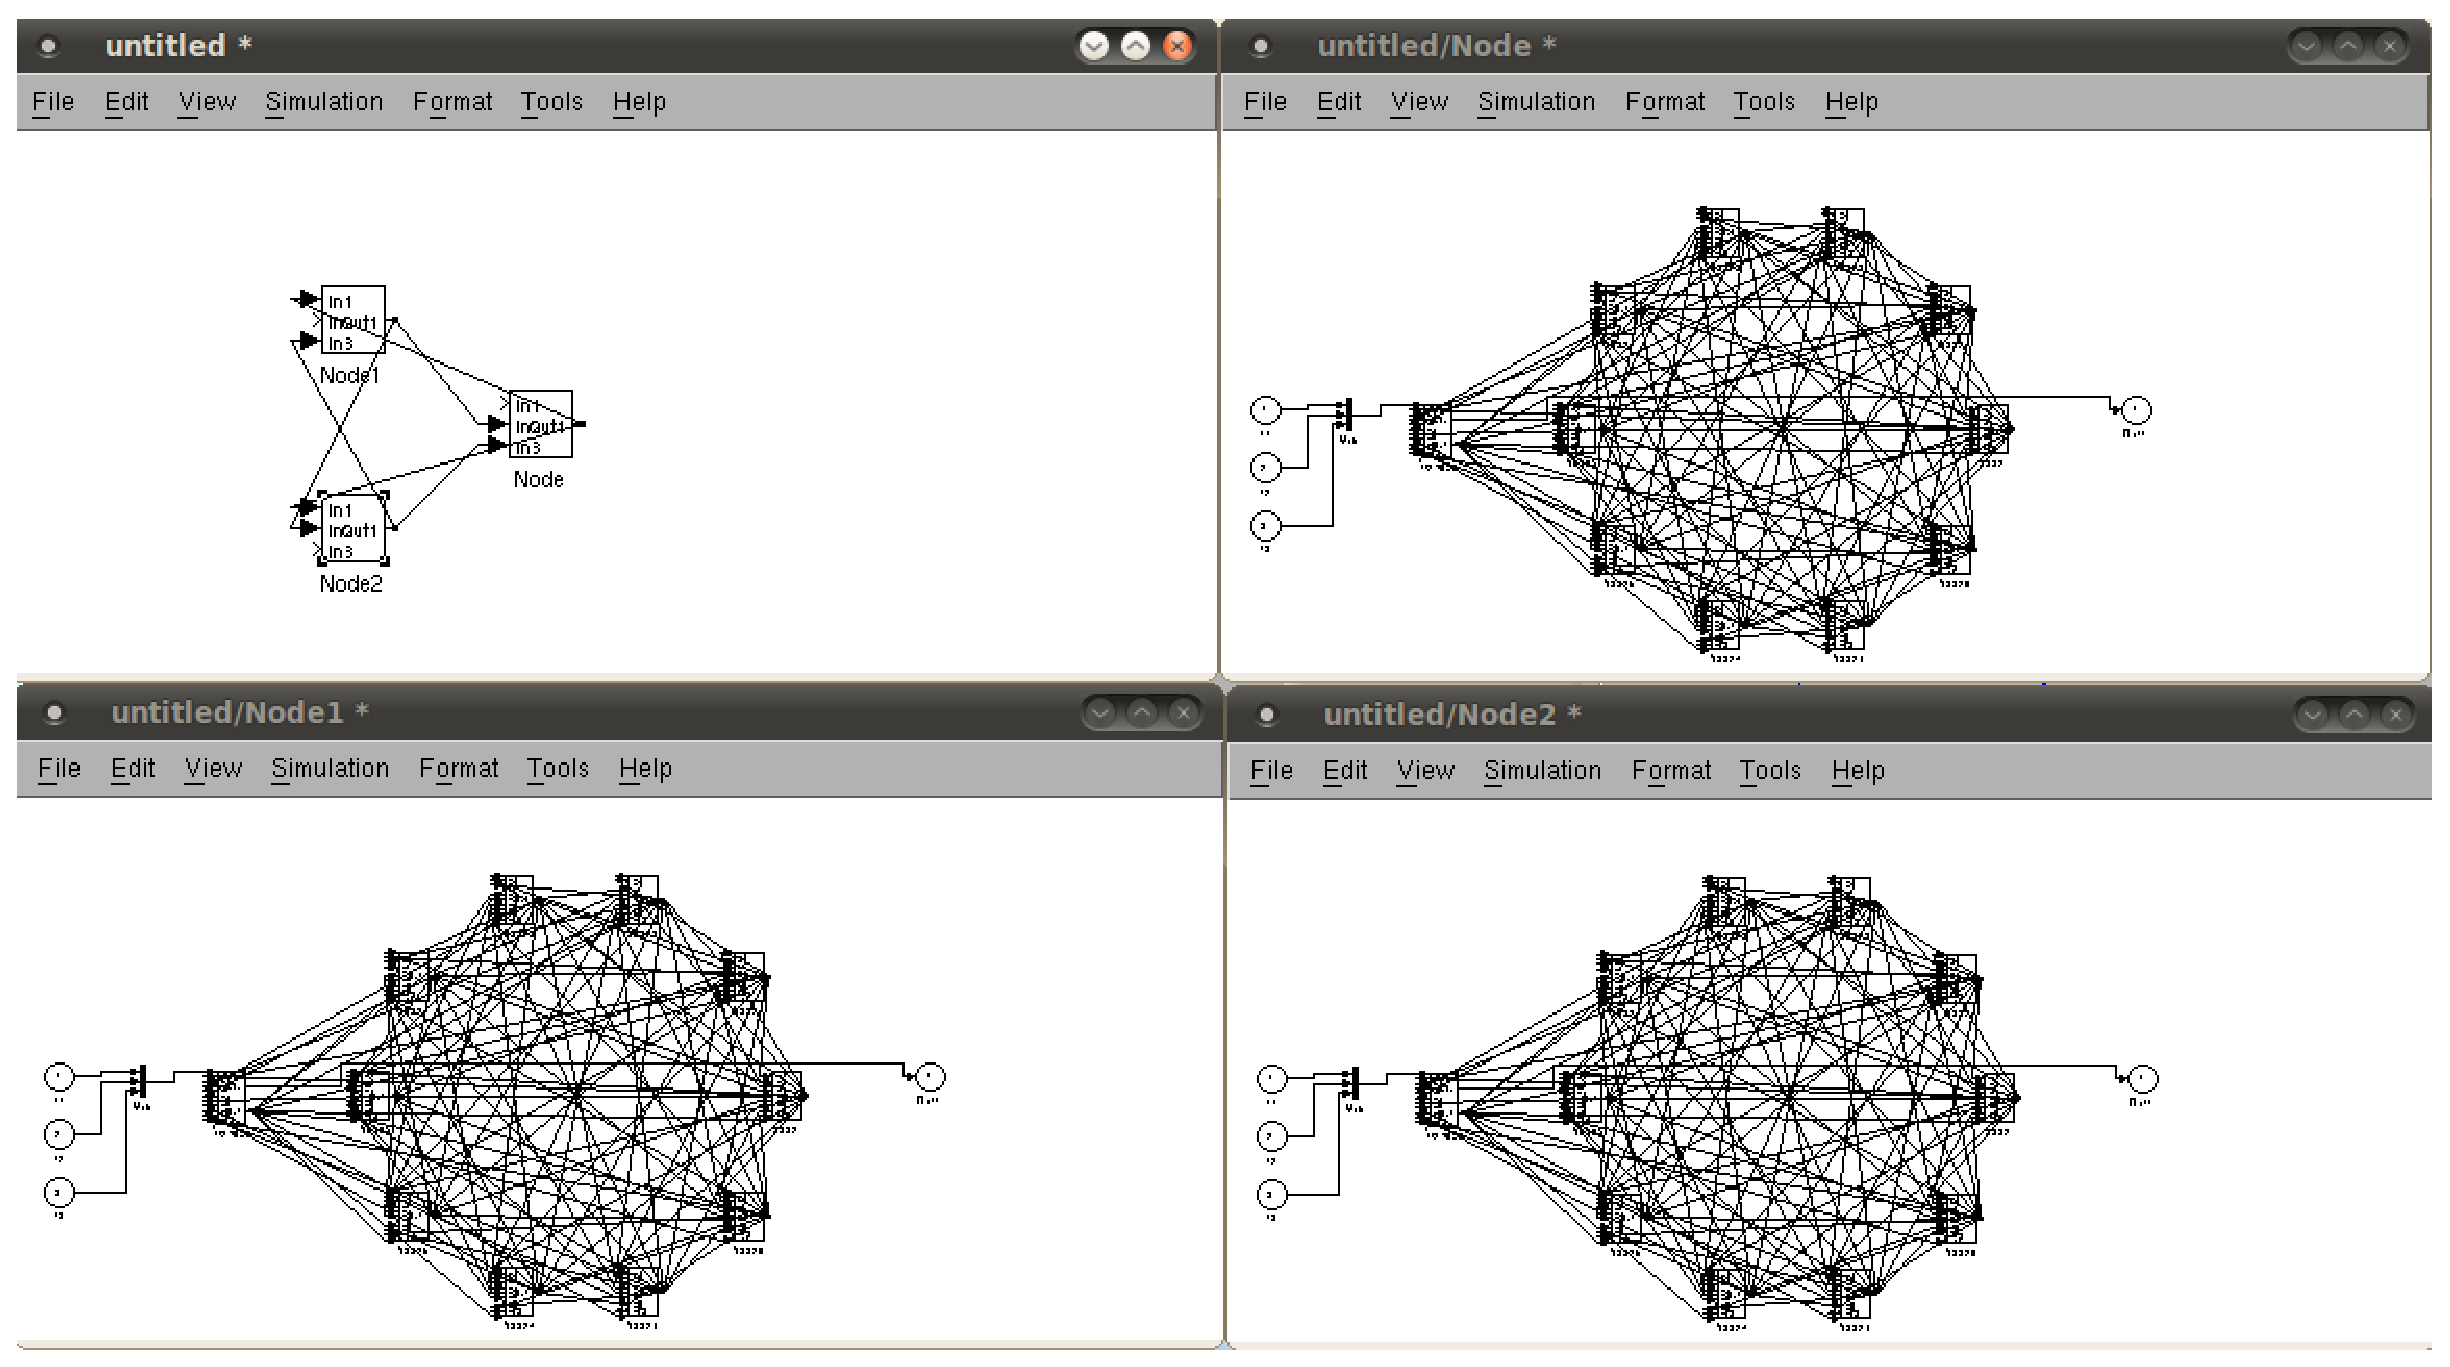
\includegraphics[width=0.5\textwidth]{pics/screenLayers.eps}
\caption[MTIDS model of layered/clustered interconnected systems]{Resulting model of layered/clustered interconnected systems. Example uses a complete graph of 3 nodes where each node is an interface/cluster of a complete graph with 10 LTI nodes plus 1 interface node.}
\label{layersFig}
\end{figure}




\subsection{Build your own Interface Node}

The user may define their own interface node behavior using the interface node template (\textbf{interfaceTemplate.mdl}). \\

\begin{figure}[htb]
\centering
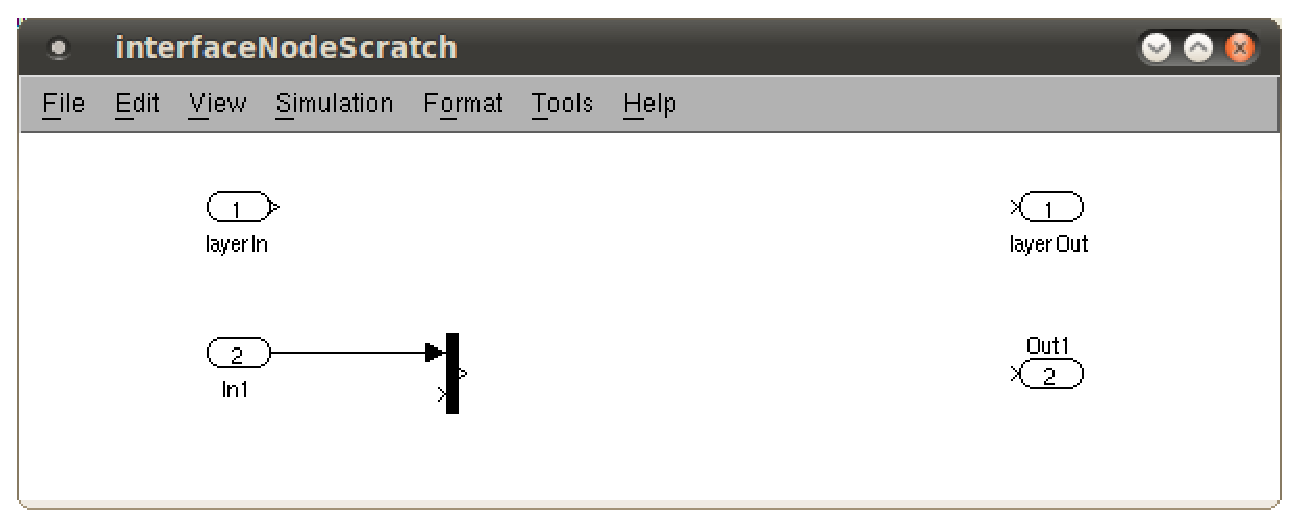
\includegraphics[width=0.5\textwidth]{pics/interfaceTemplate.eps}
\caption[MTIDS interface node template]{Interface node template model : \textbf{interfaceTemplate.mdl}.}
\label{interfaceFig}
\end{figure}
 
As we see in Figure \ref{interfaceFig} the interface node requires a layer in and out port numbered as $1$, which interacts with other layers/clusters. 
Moreover it requires the basic components of a node template (an in-port connected to a mux and an out-port) in order to interact with the nodes in the cluster/layer.
MTIDS also comes preloaded with a simple aggregating interface template called \textbf{layerInterface.mdl}.
 


 

\section{Working in Simulink}\label{workinginsimulink}

Here we review a couple of basic concepts which you will need to run and analyze the simulation of the interconnected dynamic 
systems produced by MTIDS. This is only a a refresh, for more detail please go to : \href{http://www.mathworks.com/help/toolbox/simulink/simulink_product_page.html}{Mathworks Simulink Tutorial}.

\subsection{Simulation Parameters}
The parameters of your model can be defined in Simulink by hand. However, a better way is to 
define the parameters in the Simulink model as variables and give a value to this variables in the Matlab workspace. This also allows you to save this parameters
by saving the workspace as a mat file with the command: \texttt{>> save name.mat}

\subsection{Solver} \label{solver}
Before running a simulation you need to define the simulation runtime and the numerical solver that Simulink will use to simulate your model.
In Simulink: Simulation $\rightarrow$ Configure Parameters, and then going to the solver tab, you may define different types of solver, see Figure \ref{simulink1Fig}.

\begin{figure}[htb]
\centering
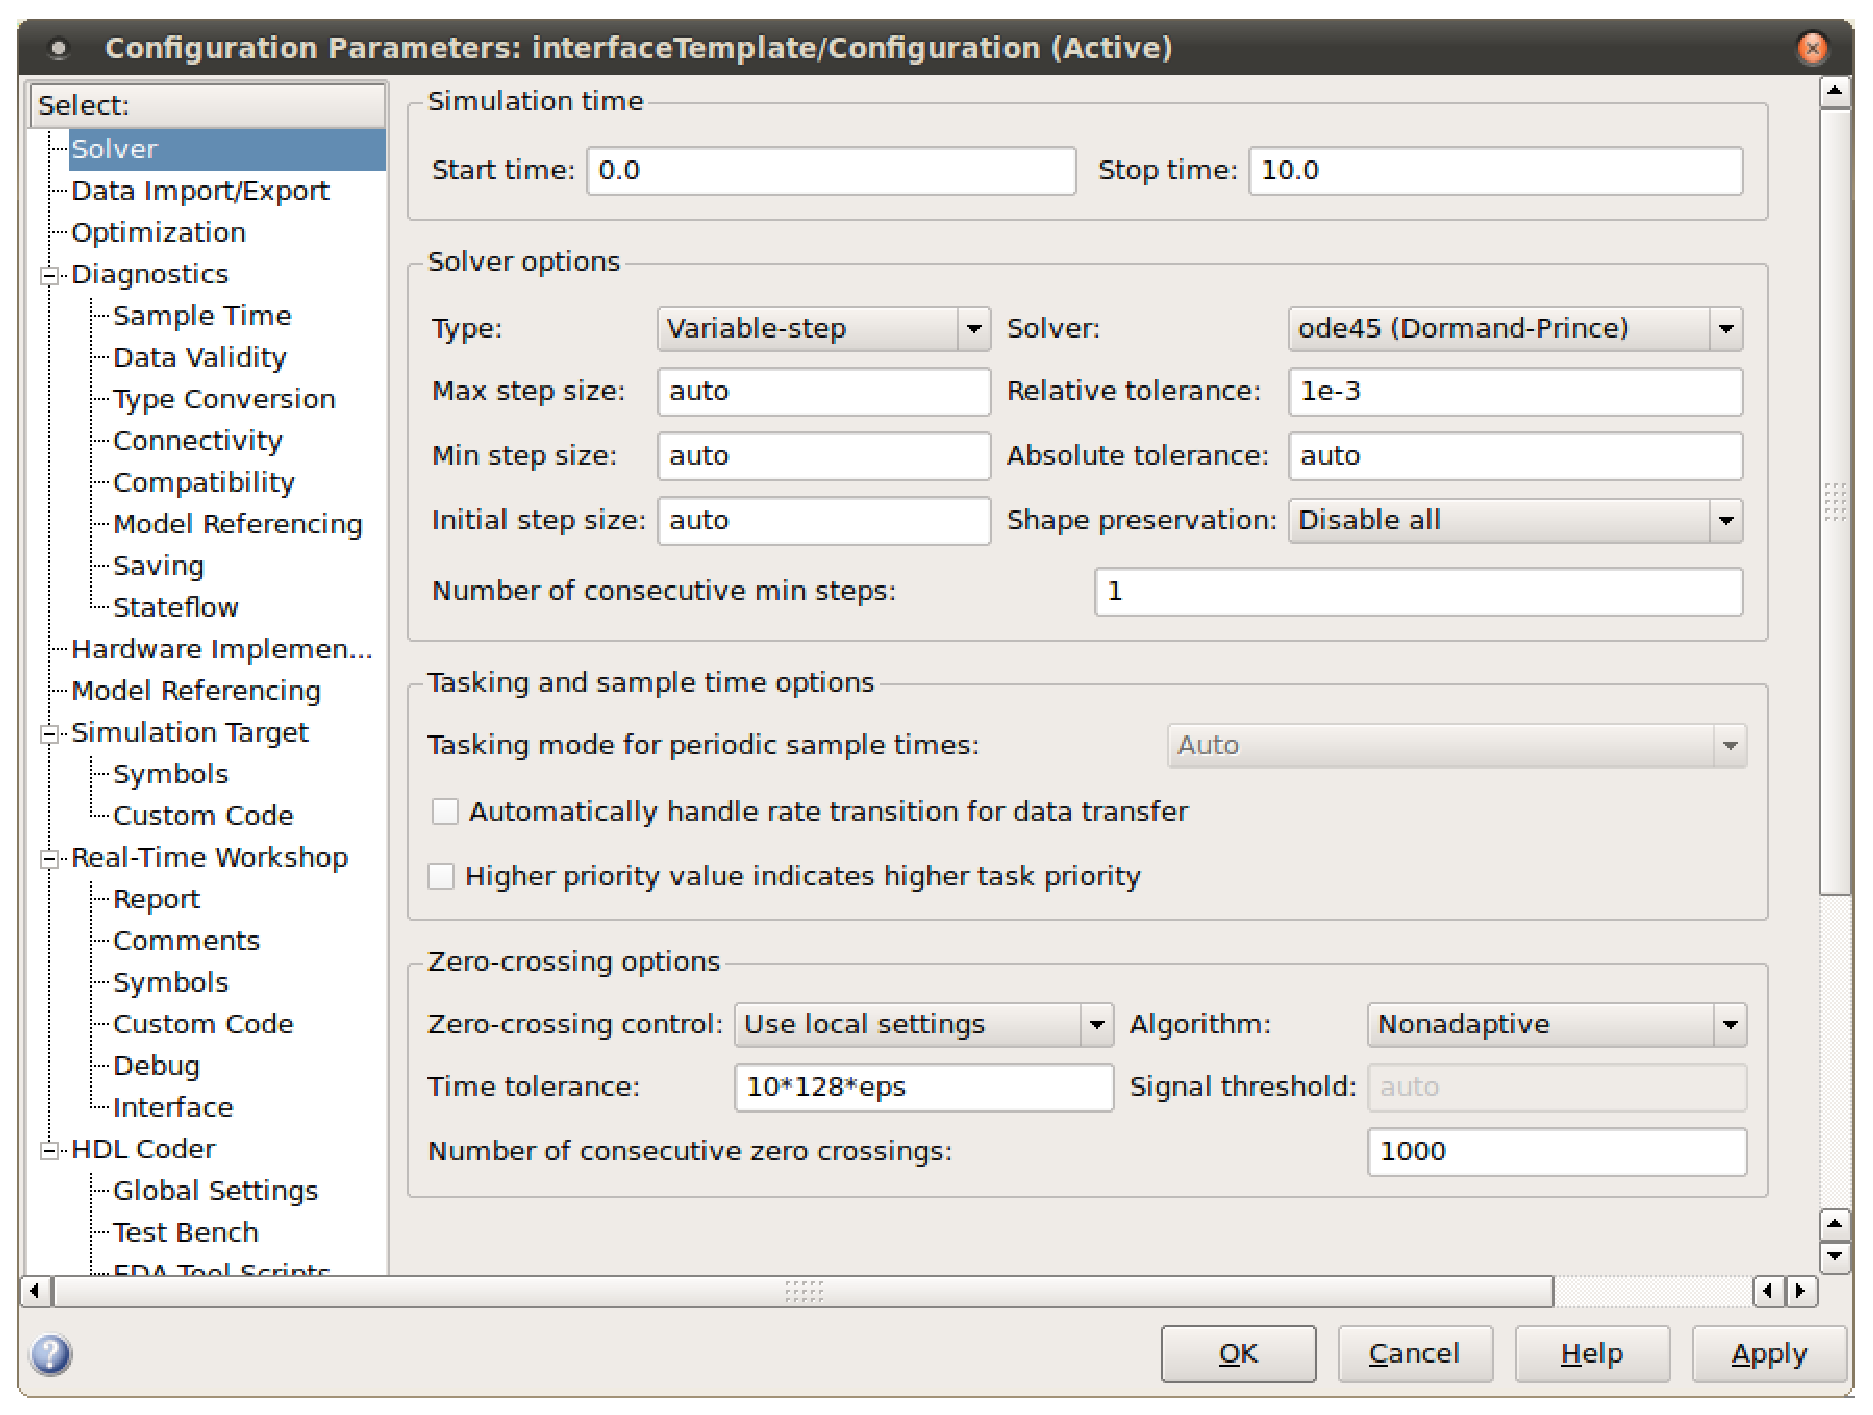
\includegraphics[width=0.5\textwidth]{pics/screenSim1.eps}
\caption[Simulink define solver]{Simulink define solver}
\label{simulink1Fig}
\end{figure} 

It is important to notice that if you want a correct time scale during simulation runtime, you need to define a fixed step size. This is used for example in the fireflies
synchronization demo.

\subsection{Visualize Simulation Data}

The easiest way to visualize data during simulations in Simulink is to use scope blocks. The data can then be seen in real-time during simulation.
Another way to do this in real-time is to use the 'To File' block or the 'To Workspace' block which allow a direct interaction with Matlab. Plotting functions can be defined in Matlab to interact with the simulation
and show the progress in real time.
\\

The other option is to visualize the result at the end of the simulation. For this you can define in Simulink which data should be send to the workspace under:
Simulation $\rightarrow$ Configure Parameters at the tab of Import/Export, see Figure \ref{simulink2Fig}. Here it is useful to export the states, which Simulink defines as the 
values coming out of integrator blocks, but it is also possible to define them by hand.

\begin{figure}[htb]
\centering
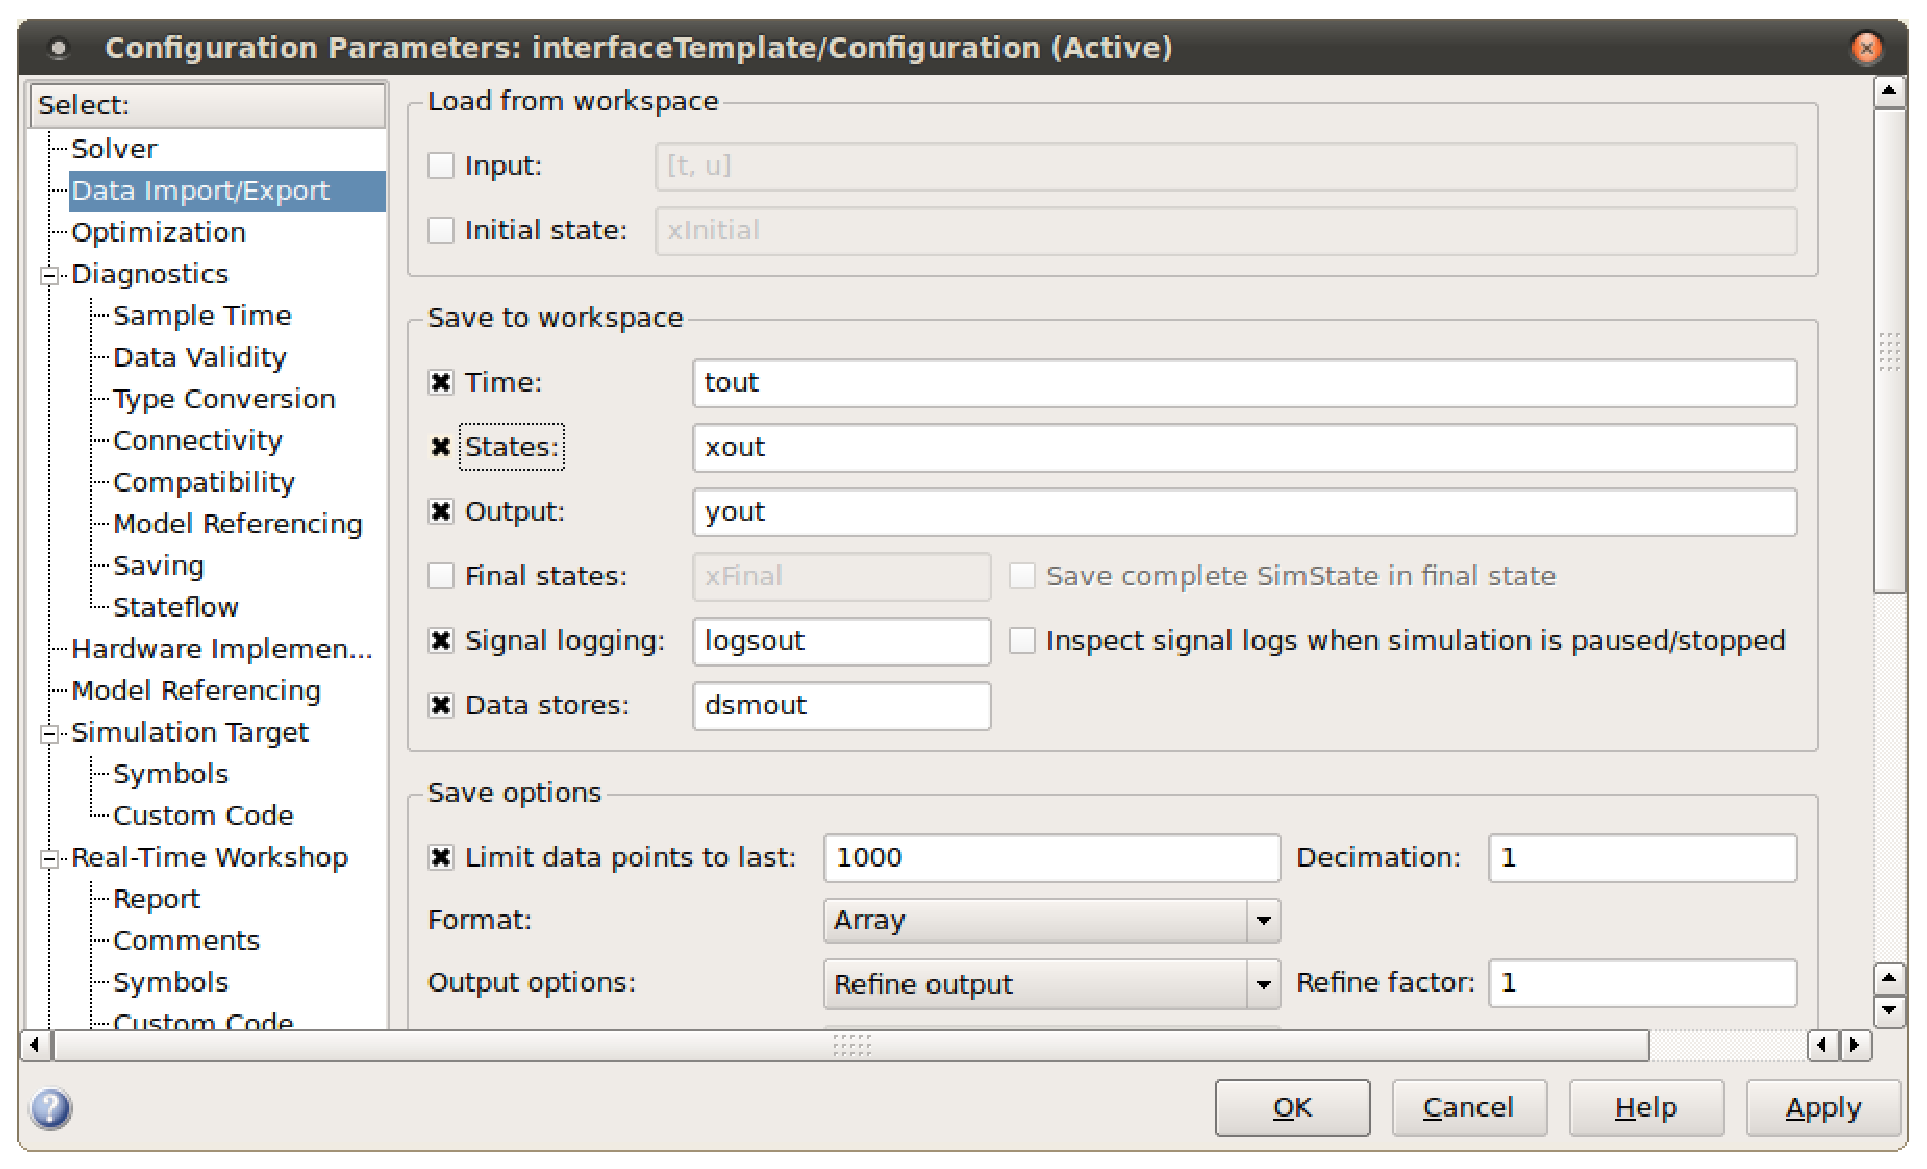
\includegraphics[width=0.5\textwidth]{pics/screenSim2.eps}
\caption[Simulink define import/export data]{Simulink define import/export data}
\label{simulink2Fig}
\end{figure} 

\subsection{Working with a closed Model}

Simulations can also be run from Matlab without the need to open the Simulink model. This is particularly useful for large Simulink models, like models of over 100 nodes that
one may produce with MTIDS. One can write a Matlab script to parametrize  and run the simulation. \textbf{Examples} can be found on the \textbf{help for the \texttt{sim} command}.
% 
% \begin{verbatim}
% Simulate the model, vdp, in Rapid Accelerator mode for an absolute tolerance 
% of 1e-5 and save the states in xoutNew and the output in youtNew.
% 
%    1. Specify parameter name-value pairs within the sim command:
% 
%       simOut = sim('vdp','SimulationMode','rapid','AbsTol','1e-5',...
%                   'SaveState','on','StateSaveName','xoutNew',...
%                   'SaveOutput','on','OutputSaveName','youtNew');
% 
%    2. Specify parameter values in a structure, paramNameValStruct:
% 
%       paramNameValStruct.SimulationMode = 'rapid';
%       paramNameValStruct.AbsTol         = '1e-5';
%       paramNameValStruct.SaveState      = 'on';
%       paramNameValStruct.StateSaveName  = 'xoutNew';
%       paramNameValStruct.SaveOutput     = 'on';
%       paramNameValStruct.OutputSaveName = 'youtNew';
%       simOut = sim('vdp',paramNameValStruct);
% 
%    3. Specify a configuration set containing the parameter values:
% 
%       mdl = 'vdp';
%       load_system(mdl)
%       simMode = get_param(mdl, 'SimulationMode');
%       set_param(mdl, 'SimulationMode', 'rapid')
%       cs = getActiveConfigSet(mdl);
%       mdl_cs = cs.copy;
%       set_param(mdl_cs,'AbsTol','1e-5',...
%                'SaveState','on','StateSaveName','xoutNew',...
%                'SaveOutput','on','OutputSaveName','youtNew')
%       simOut = sim(mdl, mdl_cs);
%       set_param(mdl, 'SimulationMode', simMode)
% \end{verbatim}
% 
% 

 


\section{Import from Simulink}

MTIDS also offers the possibility of importing Simulink models which were produced by MTIDS or are constructed following the MTIDS format, 
see section \ref{exportToSimulink}.\\

\textbf{Notice that the dynamic of the imported system node's will be the one that you have select in the MTIDS GUI.}
\\

 Node labels, position and topology is imported from Simulink to MTIDS.
To do this in MTIDS: \textbf{Simulation $\rightarrow$ Import from Simulink }, see Figure \ref{mtidsImportFig}. Finally, select the model you wish to import.

\begin{figure}[htb]
\centering
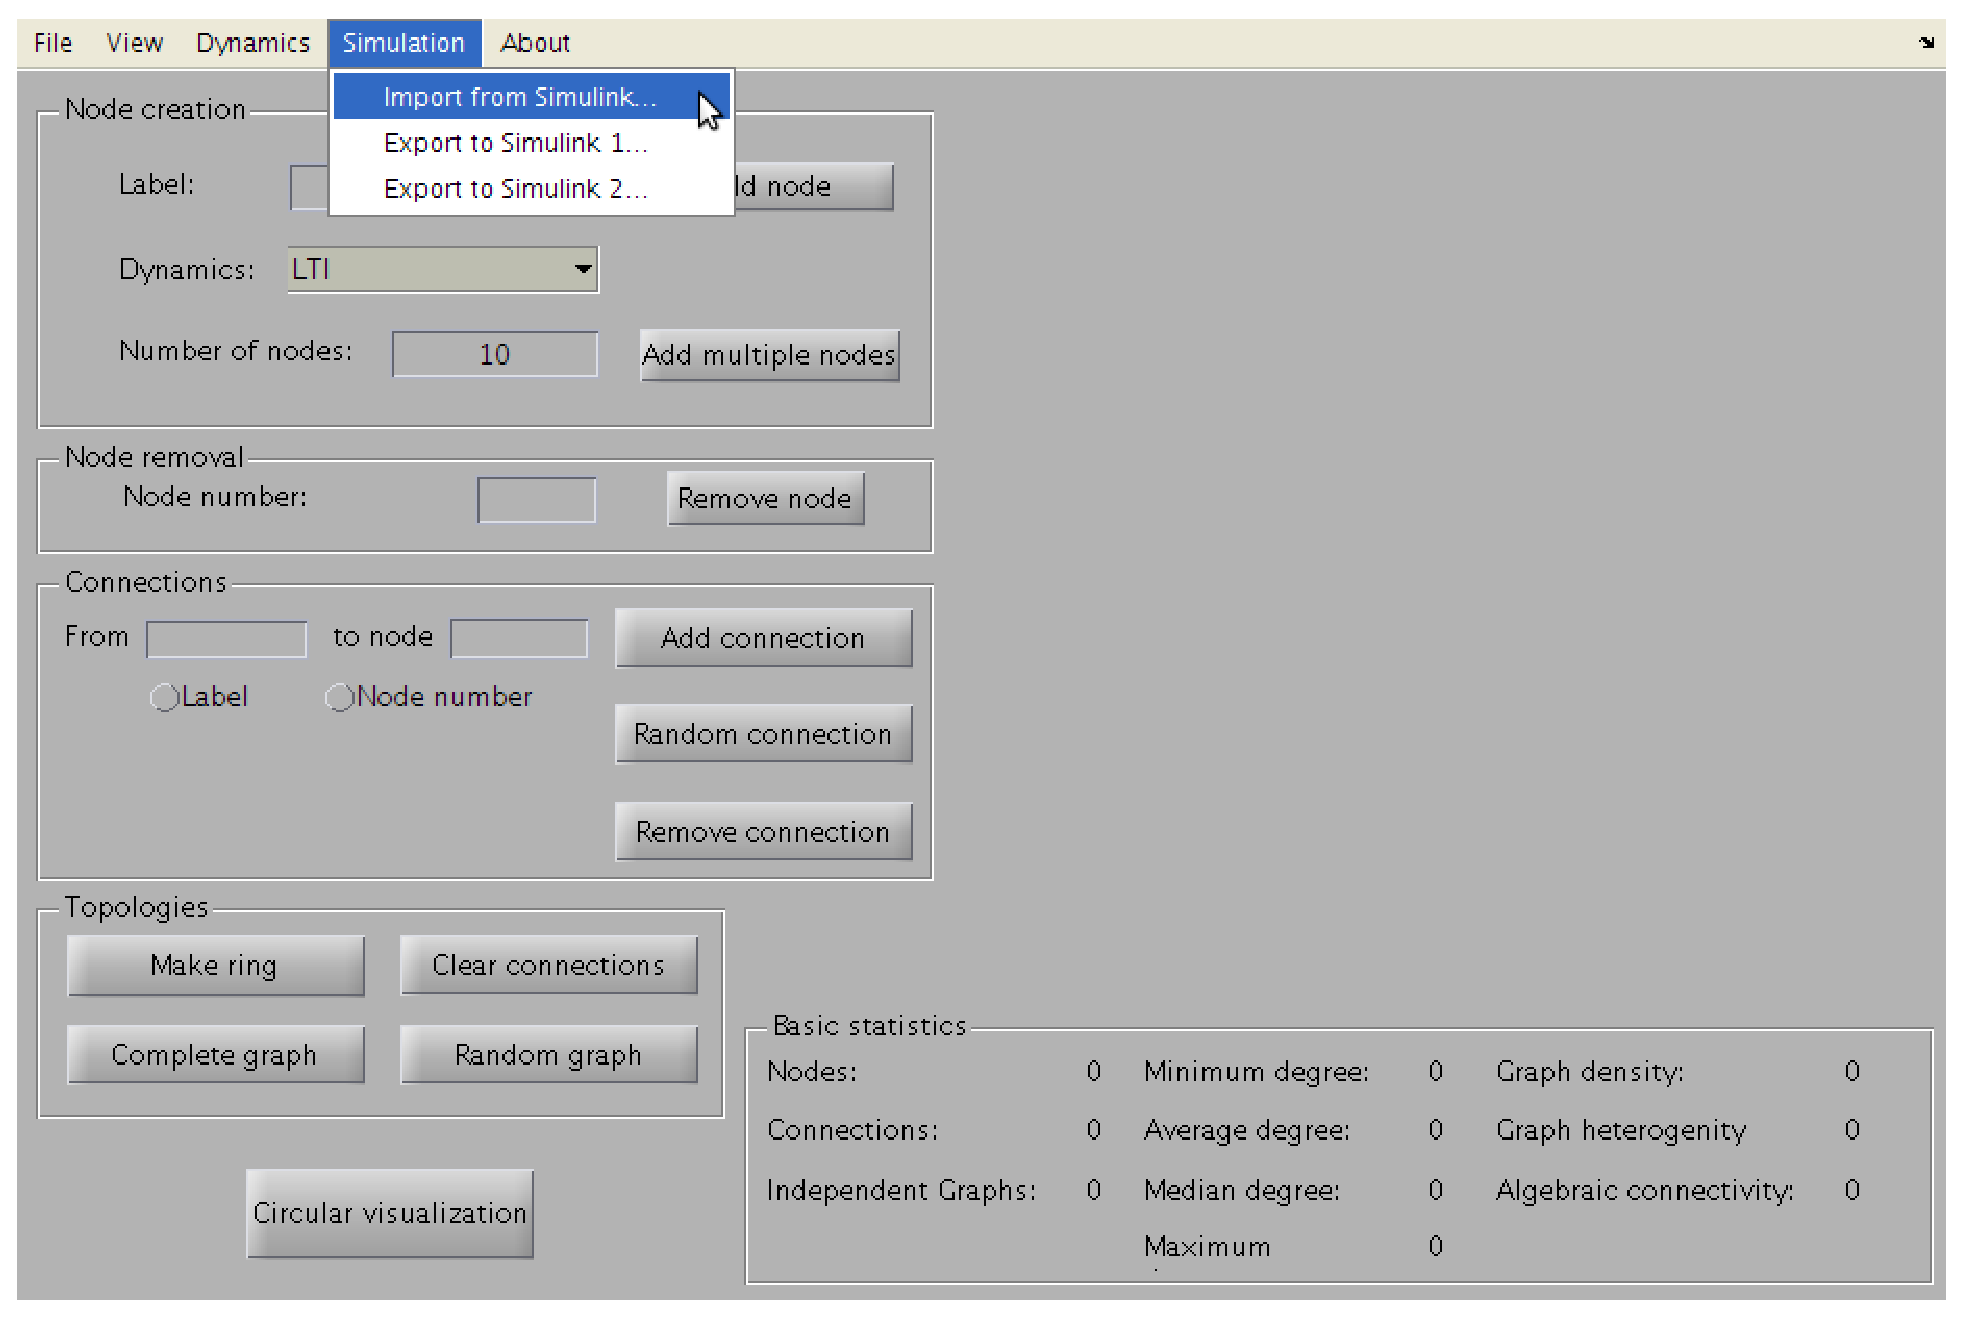
\includegraphics[width=0.5\textwidth]{pics/mtidsImport.eps}
\caption[MTIDS import form Simulink]{MTIDS import form Simulink}
\label{mtidsImportFig}
\end{figure} 



\chapter{Conclusion and Future Development}

\section{Conclusion}
In this project a toolbox for the simulation of interconnected dynamical systems was developed. MTIDS (Matlab Toolbox of Interconnected Dynamical Systems) is a wrapper that 
combines tools used for graph theory analysis (Matgraph) and the simulation of interconnected systems (Simulink) were combine to create a flexible and extensible 
framework to make the simulation of interconnected dynamical systems easier for students and researchers.\\

MTIDS offers the following \textbf{features}:
\begin{itemize}
 \item Futures....
\end{itemize}




\section{Future Development}

MTIDS is a toolbox aimed for students and researchers working in large-scale and interconnected dynamical systems. We would like to coform a community 
around this toolbox that helps push the research on this field forward.

There are still many issues and functions to improve in MTIDS:
\begin{itemize}
 \item Issues.....
\end{itemize}

%
%_______________________________________________________________


%_____Abbildungsverzeichnis_________________________________
\cleardoublepage
\addcontentsline{toc}{chapter}{List of Figures} 
\listoffigures 	 %Abbildungsverzeichnis

%___________________________________________________________
% 
% %_____Literaturverzeichnis_________________________________
% \cleardoublepage
% \addcontentsline{toc}{chapter}{Bibliography}
% \bibliography{bibliography.bib}
% \bibliographystyle{alpha}
% %__________________________________________________________


%________________Appendix_____________________________________________%


\end{document}
